% Opcje klasy 'iithesis' opisane są w komentarzach w pliku klasy. Za ich pomocą
% ustawia się przede wszystkim język i rodzaj (lic/inz/mgr) pracy, oraz czy na
% drugiej stronie pracy ma być składany wzór oświadczenia o autorskim wykonaniu.
\documentclass[declaration,shortabstract,mgr]{iithesis}

\usepackage[utf8]{inputenc}

%%%%% DANE DO STRONY TYTUŁOWEJ
% Niezależnie od języka pracy wybranego w opcjach klasy, tytuł i streszczenie
% pracy należy podać zarówno w języku polskim, jak i angielskim.
% Pamiętaj o mądrym (zgodnym z logicznym rozbiorem zdania oraz estetyka) ręcznym
% złamaniu wierszy w temacie pracy, zwłaszcza tego w języku pracy. Użyj do tego
% polecenia \fmlinebreak.
\polishtitle    {Wykrywanie i śledzenie komórek glistopodobnych w programie ImageJ}
\englishtitle   {Worm-like cell detection and tracking in ImageJ}
\polishabstract {Polskie streszczenie}
\englishabstract{English abstract}
% w pracach wielu autorów nazwiska można oddzielić poleceniem \and
\author         {Artur Rosa}
% w przypadku kilku promotorów, lub konieczności podania ich afiliacji, linie
% w poniższym poleceniu można złamać poleceniem \fmlinebreak
\advisor        {dr Andrzej Łukaszewski}
%\date          {}                     % Data złożenia pracy
% Dane do oświadczenia o autorskim wykonaniu
%\transcriptnum {}                     % Numer indeksu
%\advisorgen    {dr. Jana Kowalskiego} % Nazwisko promotora w dopełniaczu
%%%%%

%%%%% WLASNE DODATKOWE PAKIETY
%
%\usepackage{graphicx,listings,amsmath,amssymb,amsthm,amsfonts,tikz}
%
%%%%% WŁASNE DEFINICJE I POLECENIA
%
%\theoremstyle{definition} \newtheorem{definition}{Definition}[chapter]
%\theoremstyle{remark} \newtheorem{remark}[definition]{Observation}
%\theoremstyle{plain} \newtheorem{theorem}[definition]{Theorem}
%\theoremstyle{plain} \newtheorem{lemma}[definition]{Lemma}
%\renewcommand \qedsymbol {\ensuremath{\square}}
% ...

\usepackage[export]{adjustbox}
\usepackage[plain]{algorithm}
\usepackage{algorithmic}
\usepackage{amsmath}
\usepackage{graphicx}
\usepackage{qtree}
\usepackage{subcaption}

\DeclareMathOperator*{\argmax}{\textbf{argmax}}
\newcommand{\image}{\mathbf{I}}
\renewcommand{\algorithmicforall}{\textbf{for each}}

%%%%%

\begin{document}


%%%%%%%%%%%%%%%%%%%%%%%%%%%%%%%%%%%%%%%%%%%%%%%%%%%%%%%%%%%%%%%%%%%%%%%%%%%%%%%%%%%%%%%%%%%

\chapter{Wprowadzenie}

%%%%%%%%%%%%%%%%%%%%%%%%%%%%%%%%%%%%%%%%%%%%%%%%%%%%%%%%%%%%%%%%%%%%%%%%%%%%%%%%%%%%%%%%%%%


\section{Wstęp}

\ldots % TODO Wstęp

\section{Background}

\subsection{Jakich danych i do czego potrzebują biolodzy}

\ldots % TODO Jakich danych i do czego potrzebują biolodzy}

\subsection{Pozyskiwanie danych}

\ldots % TODO Pozyskiwanie danych


%%%%%%%%%%%%%%%%%%%%%%%%%%%%%%%%%%%%%%%%%%%%%%%%%%%%%%%%%%%%%%%%%%%%%%%%%%%%%%%%%%%%%%%%%%%

\chapter{Wykrywanie i śledzenie komórek}
\label{cha:detection-and-tracking}

%%%%%%%%%%%%%%%%%%%%%%%%%%%%%%%%%%%%%%%%%%%%%%%%%%%%%%%%%%%%%%%%%%%%%%%%%%%%%%%%%%%%%%%%%%%


\section{Opis problemu}
\label{sec:problem}

\subsection{Obrazy wejściowe}
\label{sec:input-images}

\ldots % TODO Obrazy wejściowe

\subsection{Pożądany efekt}
\label{sec:output}

\ldots % TODO Pożądany efekt

\section{Powiązane prace}

\ldots % TODO Powiązane prace

\section{Wykrywanie komórek}
\label{sec:cell-detection}

\subsection{Wstęp}

Problem opisany w sekcji \ref{sec:problem} zdefiniowany jest dla nagrań spod mikroskopu. Postanowiłem jednak najpierw rozwiązać podobny problem, ale zdefiniowany dla pojedynczego obrazu. Rozwiązanie tego problemu mogłoby z łatwością zostać uogólnione na stos obrazów (nagranie). W tym rozdziale opiszę rozwiązanie uproszczonego problemu: oznaczanie komórek widocznych na pojedynczym obrazie. Przez ,,oznaczenie komórki'' mam na myśli odnalezienie łamanej przechodzącej przez środek komórki, a więc jej kręgosłupa.

\subsection{Dane wejściowe}
\label{sec:detection-input}

Oznaczenie wszystkich komórek widocznych na obrazie można rozłożyć na dwa osobne problemy:
\begin{enumerate}
  \item Określenie liczby oraz lokalizacji poszczególnych komórek
  \item Odnalezienie kształtu poszczególnych komórek.
\end{enumerate}

W niniejszej pracy zdecydowałem się nie rozwiązywać automatycznie pierwszego problemu. Zamiast tego użytkownik zobowiązany jest ręcznie zaznaczyć dokładnie jeden punkt wewnątrz każdej komórki widocznej na obrazie. Wymóg ten dotyczy tylko pierwszej klatki nagrania, co opiszę dokładniej w dalszej części pracy (\ref{sec:cell-tracking}).

% TODO z którego kanału?
Danymi wejściowymi są zatem obraz $\image$ oraz zbiór punktów $\mathbf{P}$ lokalizujących komórki.

\subsection{Wybór kanału i wstępne przetwarzanie obrazu}

Obraz wejściowy składa się z dwóch podstawowych kanałów (\ref{sec:input-images}).
Chcąc jak najdokładniej oznaczyć początek i koniec komórki, a także miejsca ich podziału, postanowiłem wybrać kanał, który zawiera wyraźną informację o krawędziach w tych miejscach.
O ile kanał z fluorescencją mógłby bardzo dobrze sprawdzić się do określenie liczby oraz lokalizacji poszczególnych komórek (w przypadku ich niewielkiej liczby), o tyle drugi kanał zawiera dużo dokładniejszą informację na temat krawędzi komórek.

Celem wstępnego przetwarzania obrazu wejściowego jest w tym przypadku oddzielenie poszczególnych komórek od otoczenia, zachowując przy tym informację na temat ich krawędzi. W ramach pracy przeprowadziłem wiele testów mających na celu odnalezienie narzędzia spełniającego ten cel. Krawędzie otrzymywane za pomocą filtrów czy algorytmów do ich wyszukiwania często były nieciągłe. Dobierając inne parametry często pojawiały się niechciane zaznaczenia wewnątrz komórek.

Ostatecznie zdecydowałem się użyć narzędzia które nie jest związane z wykrywaniem krawędzi. Zaobserwowałem, że zdjęcia zrobione tą techniką mają pewne specyficzne właściwości. Komórki są na nich dość równomiernie oświetlone, przez co dobrze widać ich ,,tubowaty'' kształt. Każdą komórkę otacza też ciemne obramowanie.

\subsubsection{Mapa indeksów kształtu}

Postanowiłem spróbować wyliczyć mapę indeksów kształtu (ang. shape index map) dla obrazu wejściowego, na którym wcześniej zastosowałem rozmycie gaussowskie. Indeks kształtu to liczba z przedziału $[-1, 1]$ przyporządkowana na podstawie ,,lokalnego kształtu'' powierzchni. Jest to skaloniezminnicza (ang. scale invariant) miara, która dzieli powierzchnię na obszary wypukłe, wklęsłe i hiperboliczne (rysunek \ref{fig:shape-index-range})\cite{paper:shape-index}. Obraz wejściowy interpretowany jest tutaj jako mapa wysokości. Zastosowanie rozmycia gaussowskiego w pierwszym kroku jest niezbędne w tym przypadku ze względu na nieodporność tej miary na szum obecny na obrazie wejściowym. Do wyliczenia mapy indeksów skorzystałem z wtyczki dla programu ImageJ autorstwa Johannesa Schindelina\cite{plugin:shape-index-map}.

\begin{figure}
  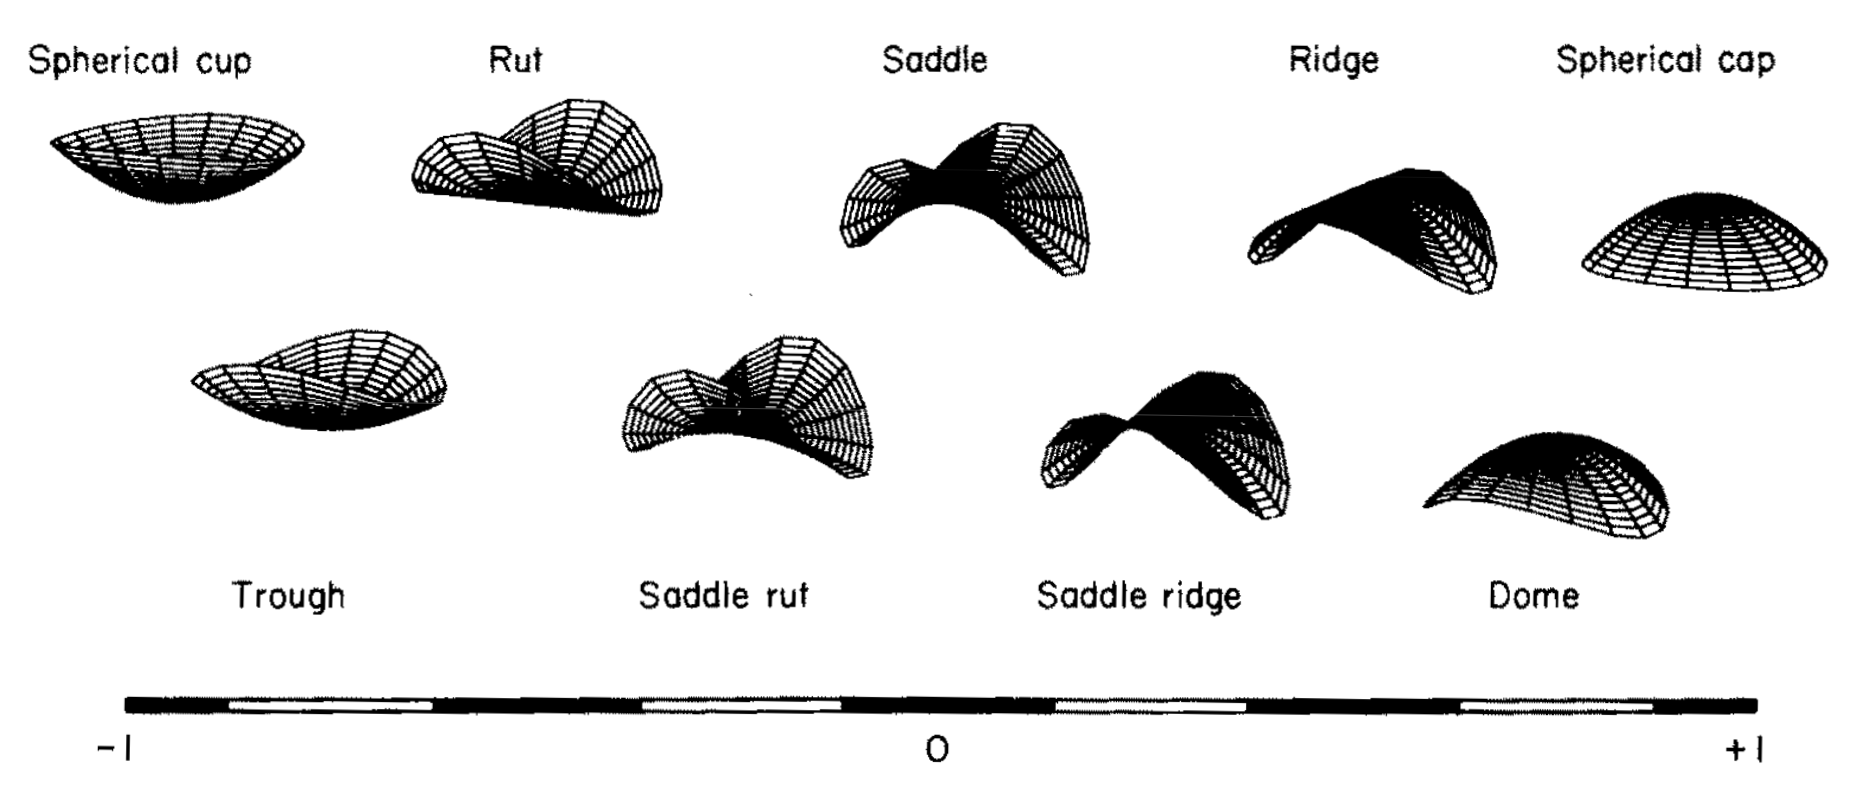
\includegraphics[width=\textwidth]{images/shape-index-range.png}
  \caption{Skala indeksu kształtu z podziałem na dziewięć kategorii. \cite{paper:shape-index}}
  \label{fig:shape-index-range}
\end{figure}

Okazało się, że na wynikowej mapie otoczenie komórek interpretowane jest jako obszar wklęsły, w przeciwieństwie do samych komórek, których wnętrze oznaczane jest indeksami kształtów wypukłych. Własność ta zachodzi na większości testowych obrazów nawet przy stosunkowo dużym zagęszczeniu komórek.

\subsection{Szkieletyzacja i wstępna detekcja komórek}

Zgodnie z powyższą obserwacją, możemy łatwo oddzielić komórkę od jej otoczenia na obrazie ustalając pewien próg $t \approx 0$. Załóżmy przez chwilę, że binaryzując w ten sposób mapę indeksów kształtu otrzymamy obraz $\image_{bin}$, na którym każdy piksel leżący wewnątrz dowolnej komórki będzie miał wartość $1$, natomiast każdy piksel należący do zewnętrznego obrysu dowolnej komórki (nie należący do komórki, lecz sąsiadujący z pikselem należącym do niej) będzie miał wartość $0$.
Przy takim założeniu każda komórka jest niezależną ,,wyspą'' na binarnym obrazie $\image_{bin}$. Chcąc odnaleźć ,,kręgosłup'' komórki (łamaną przechodzącą przez jej środek) chcemy tak naprawdę znaleźć łamaną, która jest równoodległa od jej krawędzi. Bardzo podobny problem rozwiązują algorytmy do wyznaczania szkieletu. Ich celem jest odnalezienie zbioru punktów równoodległych od co najmniej dwóch brzegów.

Na potrzeby tej pracy do szkieletonizacji użyta została implementacja algorytmu ,,3D thinning algorithm''\cite{algo:3d-thinning} w formie pluginu dla programu ImageJ\cite{plugin:skeletonize-3d}. Mimo iż wtyczka pozwala na szkieletyzację obrazów 3D, w tym przypadku została użyta do przetworzenia pojedynczego obrazu 2D. Wynikiem szkieletyzacji jest binarny obraz o pewnych właściwościach. Każdy aktywny piksel można przyporządkować do trzech grup:
\begin{itemize}
  \item końcówki -- mają mniej niż 2 sąsiadujące aktywne piksele
  \item węzły -- mają więcej niż 2 sąsiadujące aktywne piksele
  \item połączenia -- mają dokładnie 2 sąsiadujące aktywne piksele.
\end{itemize}
Przedstawiając szkielet jako graf końcówki tworzyłyby wierzchołki o stopniu równym $1$ lub $0$, wierzchołki o większych stopniach przedstawiałyby zbiory sąsiadujących ze sobą węzłów, natomiast krawędzie reprezentowałyby zbiory sąsiadujących ze sobą połączeń (zakończonych zbiorem węzłów lub końcówką). Taką reprezentację grafową można uzyskać za pomocą kolejnej wtyczki dla programu ImageJ tego samego autora\cite{plugin:analyze-skeleton}. Poza standardowymi informacjami wierzchołki i krawędzie utworzonego za jej pomocą grafu przechowują zbiory pikseli które reprezentują.

Ze względu na specyficzny kształt komórki można zaobserwować następującą właściwość: po przeprowadzeniu szkieletyzacji obrazu $\image_{bin}$, o ile przyjęte wcześniej założenie jest spełnione, szkielet każdej z komórek składa się dokładnie z dwóch końcówek i połączeń między nimi. Łamaną opisującą zbiór połączeń można z powodzeniem nazwać ,,kręgosłupem komórki''. Mając do dyspozycji zbiór punktów $\mathbf{P}$ lokalizujących komórki można teraz w łatwy sposób odnaleźć dla każdej z nich graf ją opisujący (zawierający dwa wierzchołki i jedną krawędź). Jednym ze sposobów może być wyszukanie dla każdego punktu ze zbioru $\mathbf{P}$ krawędź która znajduje się najbliżej tego punktu, gdzie odległość między punktem a krawędzią zdefiniowana jest jako odległość między punktem, a najbliższym pikselem, który należy do zbioru opisywanego przez tę krawędź.

\subsection{Wybór krawędzi w węzłach}
\label{sec:spine-extending}

Niestety przyjęte założenie o tym, że każdy piksel należący do zewnętrznego obrysu dowolnej komórki będzie miał wartość $0$, nie zawsze jest spełnione. W realistycznym scenariuszu zdarza się, że jedna z końcówek komórki znajdują się na tyle blisko innej komórki, że wstępne przetwarzanie i progowanie obrazu nie powoduje ich rozdzielenia na obrazie binarnym. Czasem artefakty widoczne na obrazie wejściowym powodują, że wyspa na obrazie binarnym zawiera nie tylko komórkę, ale także fragment innego kształtu. W zdecydowanej większości takich przypadków kręgosłup komórki można opisać spójnym podgrafem o stopniu 2 grafu reprezentującego szkielet wyspy zawierającej komórki.

Wstępna detekcja kręgosłupa danej komórki polega, tak jak w scenariuszu optymistycznym, na odnalezieniu krawędzi $\{v_0, u_0\}$ w grafie $\mathbf{G}$ leżącej najbliżej punktu opisującego komórkę, a następnie na stworzeniu z niej i jej wierzchołków nowego grafu $\mathbf{S}_0$. Tak utworzony kręgosłup rozszerzany jest później zgodnie z następującym algorytmem:

\begin{algorithm}[H]
\begin{algorithmic}
\FORALL{$v \in \{ v_0, u_0 \}$}
  \LOOP
    \STATE
      $\text{E}_v \gets$ podzbiór krawędzi grafu $E(\mathbf{G}) - E(\mathbf{S}_n)$ incydentnych do $v$,\newline
      \hphantom{$\text{E}_v \gets$} które nie tworzą cyklu w grafie $\mathbf{S}_n$
    \IF{$\text{E}_v = \O$}
      \STATE \textbf{break}
    \ENDIF
    \STATE $\{v, u\} \gets \argmax_{e \in \text{E}_v} \ q_v(e)$
    \STATE $\mathbf{S}_{n+1} \gets \mathbf{S}_n \cup (\{u\}, \{\{v, u\}\}) $
    \STATE $v \gets u$
  \ENDLOOP
\ENDFOR
\end{algorithmic}
\end{algorithm}

\noindent
Funkcja $q_v(e)$ jest tutaj funkcją oceny, która służy do wyboru najmocniej związanej krawędzi. Siła wiązania zdefiniowana jest tutaj jako najniższa wartość indeksu kształtu (oryginalnego obrazu) dla piksela leżącego na krawędzi $e$, w okolicy wierzchołka $v$ (w odległości nie większej niż pewna stała $d$ od środka masy pikseli tworzących węzeł $v$).

Takie rozwiązanie sprawdza się dobrze dla komórek, których kręgosłup znajduje się w grafie $\mathbf{G}$, oraz jego zakończenia w tym grafie mają stopień $1$. Pomijam na ten moment przypadek, gdy szukany kręgosłup komórki nie istnieje w grafie $\mathbf{G}$. W pozostałych przypadkach przynajmniej jedno z zakończeń szukanego kręgosłupa $\mathbf{S}$ ma w grafie $\mathbf{G}$ stopień większy niż $1$. Zatem, o ile funkcja oceny $q_v(e)$ sprawdzi się dobrze jeśli chodzi o dobór krawędzi należących do szukanego kręgosłupa komórki, uzyskany na końcu algorytmu kręgosłup $\mathbf{S}_n$ będzie nadgrafem szukanego kręgosłupa $\mathbf{S}$. W takim przypadku ,,nadmiarowa'' część kręgosłupa należy do szkieletu innej komórki lub jest wynikiem artefaktu widocznego na oryginalnym obrazie. Drugi przypadek pozostawiam do ręcznego rozwiązania użytkownikowi. Pierwszy natomiast, nachodzące na siebie kręgosłupy komórek, rozwiązuję automatycznie.

\subsection{Rozwiązywanie konfliktów}
\label{sec:fix-conflicts}

Rozdzielanie nachodzących na siebie komórek nazwałem ,,rozwiązywaniem konfliktów''. Niech $\mathbf{\Sigma}_0$ będzie zbiorem wszystkich znalezionych kręgosłupów, natomiast $X(\mathbf{\Sigma})$ zbiorem par kręgosłupów nachodzących na siebie należących do zbioru $\mathbf{\Sigma}$. Rozwiązywanie konfliktów przebiega w następujący sposób:

\begin{algorithm}[H]
\begin{algorithmic}

\WHILE{$X(\mathbf{\Sigma}_n) \neq \O$}
  \STATE $\{S_x, S_y\} \gets$ dowolna para ze zbioru $X(\mathbf{\Sigma})$
  \STATE $\{S_x', S_y'\} \gets$ wynik rozwiązania konfliktu pomiędzy $S_x$ i $S_y$
  \STATE $\mathbf{\Sigma}_{n+1} \gets (\mathbf{\Sigma}_n - \{S_x, S_y\}) \cup \{S_x', S_y'\}$
\ENDWHILE

\end{algorithmic}
\end{algorithm}

Sposób w jaki rozwiązywany jest konflikt pomiędzy dwoma kręgosłupami, zależy od tego w jaki sposób nachodzą one na siebie. Kluczową rolę odgrywają tutaj także punkty lokalizujące komórki. W dalszej części pisząc, o punkcie charakterystycznym komórki, będę miał na myśli punkt leżący na kręgosłupie będący najbliżej punktu lokalizującego komórkę. Wyróżniłem 4 typy nakładania się kręgosłupów.

\subsubsection{Nakładanie się częściowe z końcówką}

\begin{figure}[H]
  \centering
  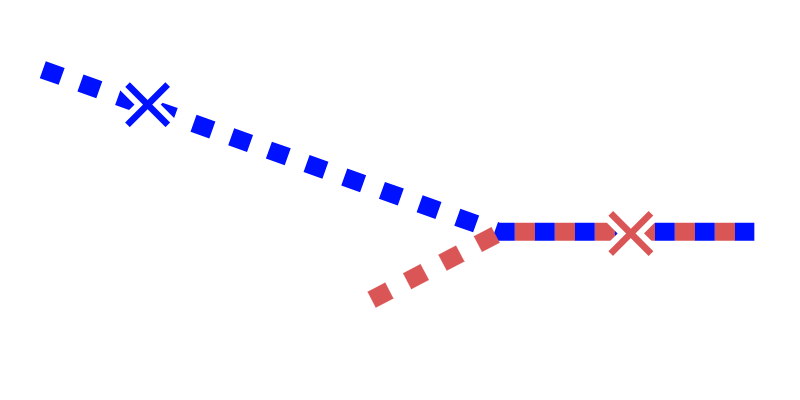
\includegraphics[valign=m,width=0.35\textwidth]{images/overlap-pwv.png}
  $\rightarrow$
  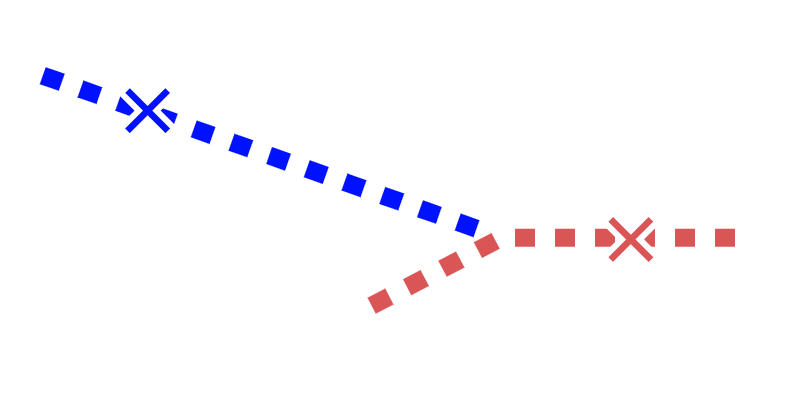
\includegraphics[valign=m,width=0.35\textwidth]{images/overlap-pwv-solved.png}
\end{figure}

W tym przypadku część wspólna przydzielana jest do jednego z kręgosłupów w całości.
Są dwie możliwości: oba punkty charakterystyczne komórki leżą poza częścią wspólną lub dokładnie jeden z nich znajduje się w części wspólnej.
Gdyby oba punkty leżały w części wspólnej, to ze względu na sposób konstrukcji szkieletów, podczas procesu rozszerzania dobierane byłyby te same krawędzie, a więc końcowo oba kręgosłupy byłyby dokładnie takie same.
W drugim przypadku sprawa jest prosta -- część wspólna zostaje przydzielona do kręgosłupa którego punkt charakterystyczny leży w części wspólnej. W pierwszym przypadku część wspólna przydzielana jest do tego kręgosłupa z którym jest mocniej związana (siłę wiązania określam w podobny sposób jak w algorytmie konstrukcji kręgosłupa).

\subsubsection{Nakładanie się częściowe}

\begin{figure}[H]
  \centering
  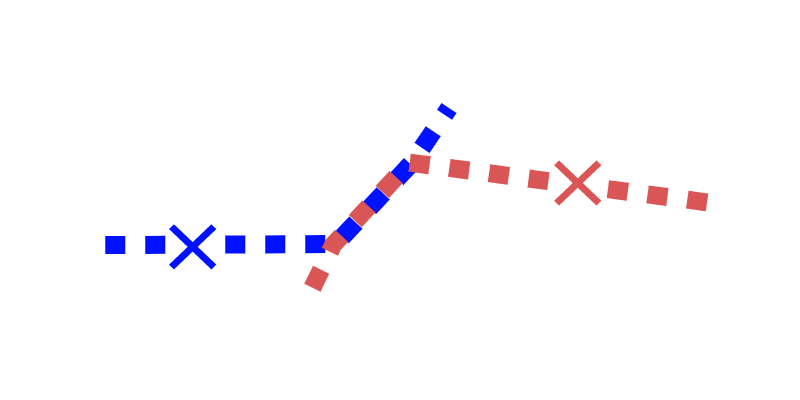
\includegraphics[valign=m,width=0.35\textwidth]{images/overlap-p.png}
  $\rightarrow$
  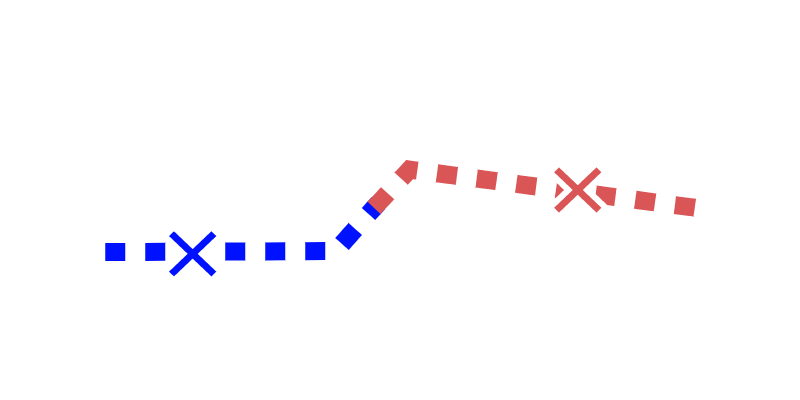
\includegraphics[valign=m,width=0.35\textwidth]{images/overlap-p-solved.png}
\end{figure}

W przypadku takiego rodzaju nakładania oba punkty charakterystyczne komórki znajdują się poza częścią wspólną.
Rozwiązanie konfliktu polega tutaj na znalezieniu najsłabszego punktu części wspólnej (mającego najniższy indeks kształtu), a następnie odpowiednim skróceniu obu kręgosłupów do tego punktu.

\subsubsection{Pełne pokrycie}

\begin{figure}[H]
  \centering
  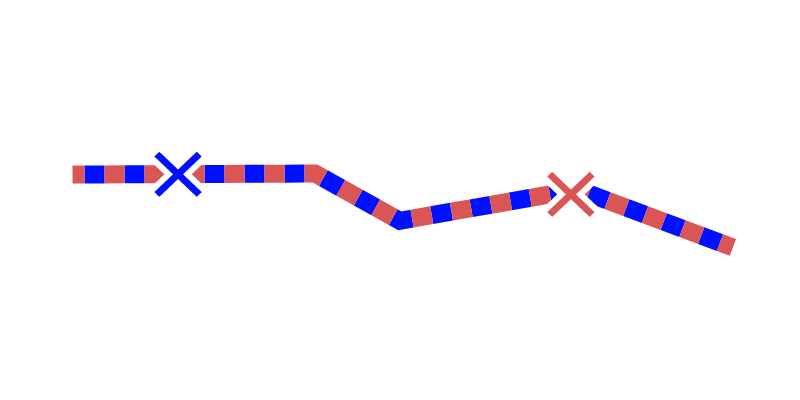
\includegraphics[valign=m,width=0.35\textwidth]{images/overlap-f.png}
  $\rightarrow$
  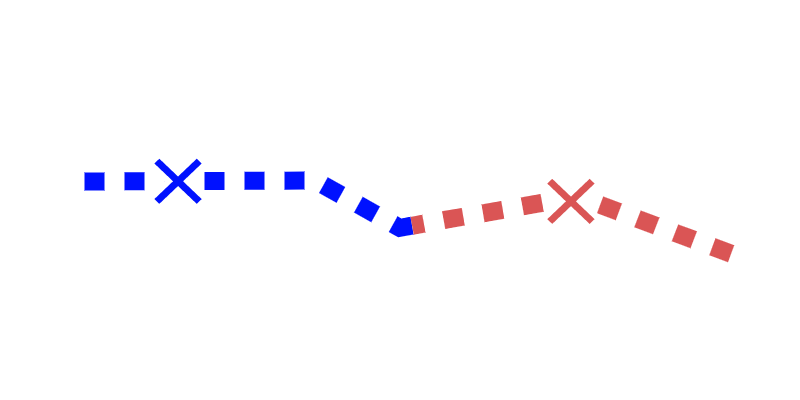
\includegraphics[valign=m,width=0.35\textwidth]{images/overlap-f-solved.png}
\end{figure}

Sposób rozwiązania tego konfliktu jest bardzo podobny do sposobu rozwiązania nakładania się częściowego. Najsłabszy punkt wyszukiwany jest w tym przypadku pomiędzy punktami charakterystycznymi komórek.


\subsubsection{Nakładanie się wielokrotne}

\begin{figure}[H]
  \centering
  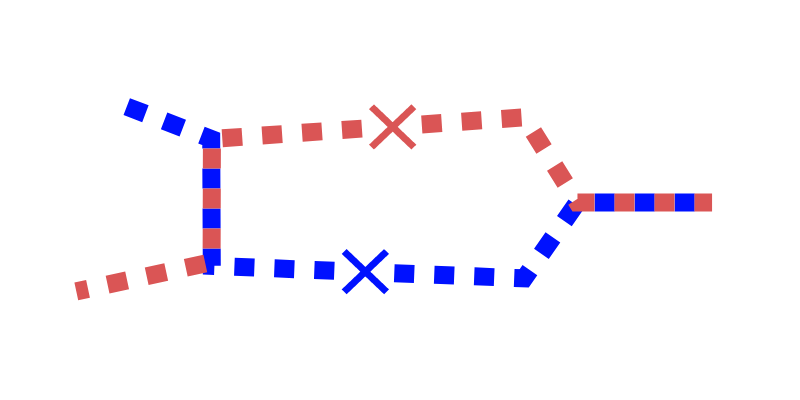
\includegraphics[valign=m,width=0.3\textwidth]{images/overlap-m.png}
  $\rightarrow$
  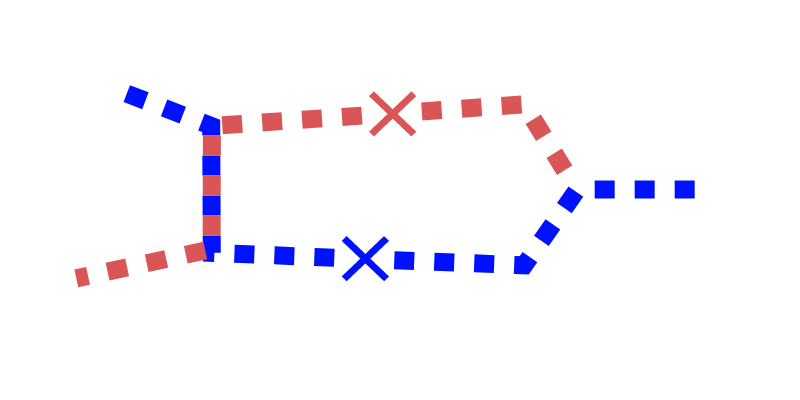
\includegraphics[valign=m,width=0.3\textwidth]{images/overlap-m-solved1.png}
  $\rightarrow$
  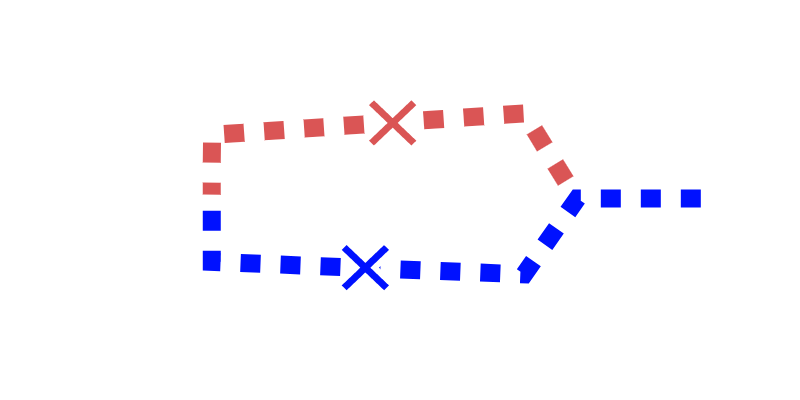
\includegraphics[valign=m,width=0.3\textwidth]{images/overlap-m-solved2.png}
\end{figure}

Dwa kręgosłupy mogą mieć więcej niż jeden konflikt równocześnie. Jest to rzadkie, ale realistyczne.
W tym przypadku w każdej iteracji rozwiązywany jest jeden z takich konfliktów za pomocą sposobów opisanych powyżej.

\subsection{Uzyskiwanie linii łamanej korekta końcowa}

Po rozwiązaniu wszystkich konfliktów każdy kręgosłup opisuje szkielet pewnej komórki.
Kolejnym krokiem jest konwersja reprezentacji grafowej (która zawiera zbiór pikseli opisujących szkielet) do linii łamanaj.
W takiej formie użytkownik będzie mógł ręcznie modyfikować zaznaczenia komórek korzystając ze standardowego interfejsu programu ImageJ.
Pierwsza wersja linii łamanej powstaje ze wszystkich punktów tworzących krawędzie i końcówki kręgosłupa, a także ze środków masy jego węzłów.
Następnie geometria łamanej jest upraszczana za pomocą algorytmu Ramera--Douglasa--Peuckera\cite{algo:ramer-douglas-peucker}.
Algorytm ten eliminuje punkty, których usunięcie nie wpływa znacząco na kształt łamanej tj. po ich usunięciu odległość uproszczonej łamanej od oryginalnej jest nie większa niż pewna przyjęta stała.

\subsection{Korekta końcówek}
\label{sec:correct-endpoints}

Ostatnim krokiem oznaczania komórek jest korekta końcówek.
Potrzeba korekty wynika z algorytmu szkieletyzacji.
Proces ten polega na erodowaniu binarnego obrazu --- z tego powodu końcówki szkieletu komórki często oddalone są od faktycznej krawędzi na oryginalnym obrazie.
Dotyczy to tylko zakończeń które reprezentowane są przez wierzchołki mające w oryginalnym szkielecie obrazu stopień równy $1$.
Nie dzieje się tak w przypadku, gdy binarny obraz komórki łączy się w tym miejscu z inną komórką, a zakończenie powstało na skutek rozwiązania konfliktu.

Właściwej lokalizacji zakończenia komórki szukam na półprostej tworzonej przez ostatni odcinek łamanej, która ją opisuje.
Mając do dyspozycji obraz binarny na podstawie którego powstał szkielet, szukam zakończenia wyspy leżącego najbliżej początku półprostej.
Jeśli punkt ten leży nie dalej niż pewna przyjęta stała, staje się on nowym zakończeniem łamanej.
Stała którą przyjąłem była nie większa niż przewidywana szerokość komórki.

Proces ten powtarzany jest dla każdego zakończenia komórki wymagającego poprawienia.

\section{Śledzenie komórek w czasie}
\label{sec:cell-tracking}

Do tej pory opisywałem sposób na wykrywanie i oznaczanie komórek na pojedynczym obrazie, mając do dyspozycji punkty lokalizujące komórki wprowadzone przez użytkownika.
Oryginalny problem dotyczył jednak stosu obrazów przedstawiającego proces rozwoju komórek w czasie.
Uogólnienie opisanego sposobu polega na automatycznym wyznaczaniu dla każdej komórki kilku potencjalnych punktów ją lokalizujących, na podstawie łamanej opisującej tę komórkę w poprzedniej klatce nagrania naniesionej na aktualną klatkę.
Następnie wybierane są te punkty (i stworzone przez nie kręgosłupy), które dały najlepsze efekty względem pewnej funkcji oceny.

Jeśli nowy kręgosłup komórki jest znacząco krótszy niż łamana opisująca ją na poprzednim obrazie, prawdopodobnie oznacza to, że nastąpił podział komórki. W takim przypadku wyszukiwany jest kolejny kręgosłup. Tym razem kandydatów na punkty lokalizujące poszukuję tylko po jednej stronie łamanej. Jeśli pierwszy kręgosłup powstał na podstawie punktu leżącego bliżej końca łamanej, jego bliźniaczy kręgosłup prawdopodobnie znajduje się bliżej jej początku i vice versa.

Po odnalezieniu wszystkich nowych kręgosłupów zgodnie z powyższą procedurą, następuje etap rozwiązywania konfliktów, konwersji na linie łamane i ostatecznej korekty końcówek (\ref{sec:fix-conflicts}--\ref{sec:correct-endpoints}).



Niech $\mathbf{C}_n$ będzie zbiorem łamanych opisujących komórki na $n$-tym obrazie stosu.
Niech $\phi_\sigma(d)$ będzie funkcją która liczbą z przedziału $[0, 1]$ przyporządkowuje punkty leżące na łamanej $\sigma$, proporcjonalnie do odległości od jej początku (przyjmijmy, że linia łamana ma zdefiniowany ,,kierunek'', tzn. ma początek i koniec). Niech $S_n(p)$ będzie szkieletem komórki wyznaczonym zgodnie z metodą opisaną wcześniej (\ref{sec:detection-input}--\ref{sec:spine-extending}) dla punktu lokalizującego $p$ i $n$-tej klatki nagrania.
Cały proces można zobrazować następującym algorytmem:

\begin{algorithm}[H]
\begin{algorithmic}

\FORALL{$n \in \{ 0, 1, \ldots, n-1 \}$}
  \STATE $\mathbf{\Sigma}_{n+1} \gets \O$
  \FORALL{$\sigma \in \mathbf{C}_n$}
    \STATE $\Sigma \gets \{ S_{n+1}(\phi_\sigma(d)) \ | \ d \in \text{D} \}$
    \STATE $S \gets \argmax_{S \in \Sigma} \ q_\sigma(S)$
    \STATE $\mathbf{\Sigma}_{n+1} \gets \mathbf{\Sigma}_{n+1} \cup \{ S \}$
    
    \IF{$| S | < 0.9 \cdot | \sigma |$}
      \STATE $\Sigma' \gets \{ S_{n+1}(\phi_\sigma(d')) \ | \ d' \in \text{D}' \}$
      \STATE $S' \gets \argmax_{S' \in \Sigma} \ q_\sigma(S')$
      \STATE $\mathbf{\Sigma}_{n+1} \gets \mathbf{\Sigma}_{n+1} \cup \{ S' \}$
    \ENDIF
  \ENDFOR
  \STATE $\mathbf{\hat{\Sigma}}_{n+1} \gets$ wynik rozwiązania konfliktów w zbiorze $\mathbf{\Sigma}_{n+1}$
  \STATE $\mathbf{C}_{n+1} \gets$ wynik konwersji na łamane i korekcie końcówek elementów zbioru $\mathbf{\hat{\Sigma}}_{n+1}$
\ENDFOR

\end{algorithmic}
\end{algorithm}

\noindent
W algorytmie pojawia się zbiór $D \subseteq [0, 1]$ którego elementy dobrałem empirycznie jako $\{ 0.2, 0.4, 0.6, 0.8 \}$.
Zbiór $D' \subset D$ to zbiór, który zależy od wcześniejszego wyboru najlepszego kandydata na kręgosłup komórki. Jeśli w danej iteracji kręgosłup $S$ powstał na podstawie punktu lokalizującego leżącego na pierwszej połowie łamanej, będzie to zbiór $\{ d \in D \ | \ d > 0.5 \}$ w przeciwnym wypadku będzie to pozostała część zbioru $D$.

\section{Interakcja ze strony użytkownika}

Niestety powyższe działania nie sprawdzą się dobrze w każdym przypadku.
Jest wiele czynników które utrudniają poprawną detekcję komórek.
Większość z nich związana jest ze słabą jakością nagrań.
Obrazy są mocno zaszumione, często występują na nich artefakty, czasem płytka na której poruszają się komórki minimalnie się przesuwa, a innym razem mikroskop traci ostrość na kilka klatek nagrania.
Zapewne można próbować rozwiązać te problemy automatycznie, ale na pewno pojawią się nowe, nie rozważane wcześniej przypadki.
Właśnie z tego powodu postanowiłem zapewnić użytkownikowi możliwość interaktywnego poprawiania automatycznie wyznaczonych komórek, ale także całkowicie manualne kontynuowanie detekcji, zachowując przy tym informacje o historii komórek.

Komórki przedstawione są w oknie programu jako standardowe zaznaczenia programu ImageJ i można je edytować za pomocą standardowego interfejsu.
Poza tym plugin stworzyłem dwa dodatkowe narzędzia dla użytkownika.
Pierwsze z nich służy do rozcinania komórek w miejscach, w których się one dzielą.
Mimo że algorytm śledzenia ma mechanizm odpowiedzialny za zauważenie takich zmian, zdarza się że dzieje się to zbyt późno (komórki jeszcze przez pewien czas po podziale znajdują się bardzo blisko siebie).

Drugie narzędzie służy do skracania końcówek zaznaczeń.
Zauważyłem, że częstym problemem jest to, że zaznaczenie wybiega poza krawędzie komórki.
Najczęściej dzieje się to ze względu na występujące na obrazie artefakty lub punkty stałe na płytkach znajdujące się blisko zakończeń komórek.
Żeby przyspieszyć proces poprawiania takich zaznaczeń można skorzystać z narzędzia do skracania końcówek, które działa podobnie do ,,gumki'' w popularnych programach graficznych.

Chcąc ręcznie oznaczyć komórki w kolejnej klatce (zamiast wyliczać je automatycznie na podstawie poprzedniej), użytkownik może skorzystać z opcji duplikowania klatki. Dzięki temu w aktualnej klatce pojawią się wszystkie zaznaczenia z klatki poprzedniej, które następnie można ręcznie dopasować do ich nowej pozycji.


%%%%%%%%%%%%%%%%%%%%%%%%%%%%%%%%%%%%%%%%%%%%%%%%%%%%%%%%%%%%%%%%%%%%%%%%%%%%%%%%%%%%%%%%%%%

\chapter{Opis implementacji}

%%%%%%%%%%%%%%%%%%%%%%%%%%%%%%%%%%%%%%%%%%%%%%%%%%%%%%%%%%%%%%%%%%%%%%%%%%%%%%%%%%%%%%%%%%%


\section{Kod źródłowy}

Kod źródłowy projektu zamieszczony został w publicznie dostępnym repozytorium w serwisie GitHub.
% TODO Licencja?
Repozytorium można znaleźć pod adresem
\linebreak\url{https://github.com/rossinek/cell-detector-imagej-plugin}.

Program zaimplementowany jest jako wtyczka do programu ImageJ, napisana w języku Java. Do automatyzacji procesu budowy wykorzystany został Apache Maven. Wszystkie zależności zostały uwzględnione w pliku konfiguracyjnym dla Mavena, który odpowiada również za ich pobranie.

Plugin był rozwijany głównie na systemie macOS Catalina, ale został również przetestowany na systemie Windows 10. 

\section{Kompilacja i uruchomienie}

Do poprawnego zbudowania pluginu z kodu źródłowego należy upewnić się że zainstalowane są wymagane zależności. Poniższa instrukcja zakłada, że system wyposażony jest w:

\begin{itemize}
  \item Apache Maven w wersji większej lub równej \texttt{3.3.9}
  \item Java w wersji 8.
\end{itemize}

Aby zbudować projekt należy skorzystać z komendy \texttt{mvn}, która spowoduje pobranie wszystkich zależności,  kompilację kodu źródłowego i wywołanie testów automatycznych.

Zbudowany plugin dla programu ImageJ można znaleźć w folderze \texttt{target} pod nazwą \texttt{Mtbt\_Plugin-\{wersja\}.jar}. Tak spakowany plugin można zainstalować w programie ImageJ (lub Fiji) wklejając go do folderu \texttt{jars} w miejscu gdzie zainstalowany jest program.

Aby uruchomić plugin w ramach własnej niezależnej instancji ImageJ, po zbudowaniu projektu można uruchomić główną metodę programu komendą
\linebreak\texttt{mvn exec:java -Dexec.mainClass="dev.mtbt.Main"}.


\section{Obsługa pluginu}
\label{sec:user-manual}

Po zainstalowaniu pluginu w programie ImageJ pojawi się nowe menu \texttt{Development} (rysunek \ref{fig:ui-menu}) w którym znajdują się narzędzia zaimplementowane na potrzeby tej pracy. Poza głównym pluginem (\texttt{Cell detector}) znajdują się tam jeszcze dodatkowe wtyczki służące do importu oraz eksportu komórek, a także narzędzia pomocne w rozwoju programu.
\begin{figure}
  \centering
  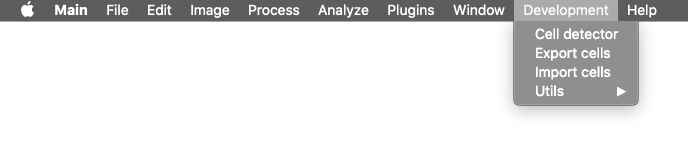
\includegraphics[width=0.7\textwidth]{images/ui-menu.png}
  \caption{Menu programu ImageJ rozszerzone o wtyczki zaimplementowane na potrzeby tej pracy.}
  \label{fig:ui-menu}
\end{figure}
Główny plugin podzielony jest na trzy kroki:


\begin{enumerate}
  \item Lokalizacja i wstępna detekcja komórek
  \item Śledzenie komórek w czasie
  \item Analiza danych
\end{enumerate}

Przed uruchomieniem pluginu należy otworzyć nagranie które chcemy analizować. Po jego uruchomieniu zobaczymy okno pluginu przedstawiające pierwszy krok.
Interfejs pluginu na każdym etapie składa się z kilku stałych i kilku zmiennych (w zależności od aktualnego kroku) części składowych.
Po prawej stronie znajduje się zawartość standardowego okna wielokanałowego stosu obrazów ImageJ.
Dwa suwaki w dolnej części służą do wyboru kanału oraz klatki nagrania.
Wybór kanału ma wpływ na to, na którym kanale odbywa się detekcja.
% TODO który kanał należy wybrać
Obok suwaka do wyboru klatki znajduje się przycisk start/stop służący do odtwarzania nagrania.
W górnej części panelu znajdującego się po lewej stronie znajdują się kontrolki specyficzne dla danego kroku pluginu. W jego dolnej części znajdują się narzędzia przydatne na każdym etapie działania pluginu, a także przyciski do zmiany kroku.


\subsection{Lokalizacja i wstępna detekcja komórek}

Pierwszy etap polega na zaznaczeniu przez użytkownika punktów lokalizujących komórki, a następnie uruchomieniu wstępnej detekcji (rysunek \ref{fig:ui-step-detector}).
W tym celu należy wcisnąć przycisk \texttt{Select cells}, zaznaczyć każdą komórkę widoczną na pierwszej klatce nagrania klikając w nią kursorem, a następnie wcisnąć przycisk \texttt{Run detection}.
W celu poprawienia wstępnej selekcji można skorzystać z przycisku \texttt{Reset}, który usuwa cały uzyskany do tej pory efekt.

\begin{figure}
  \centering
  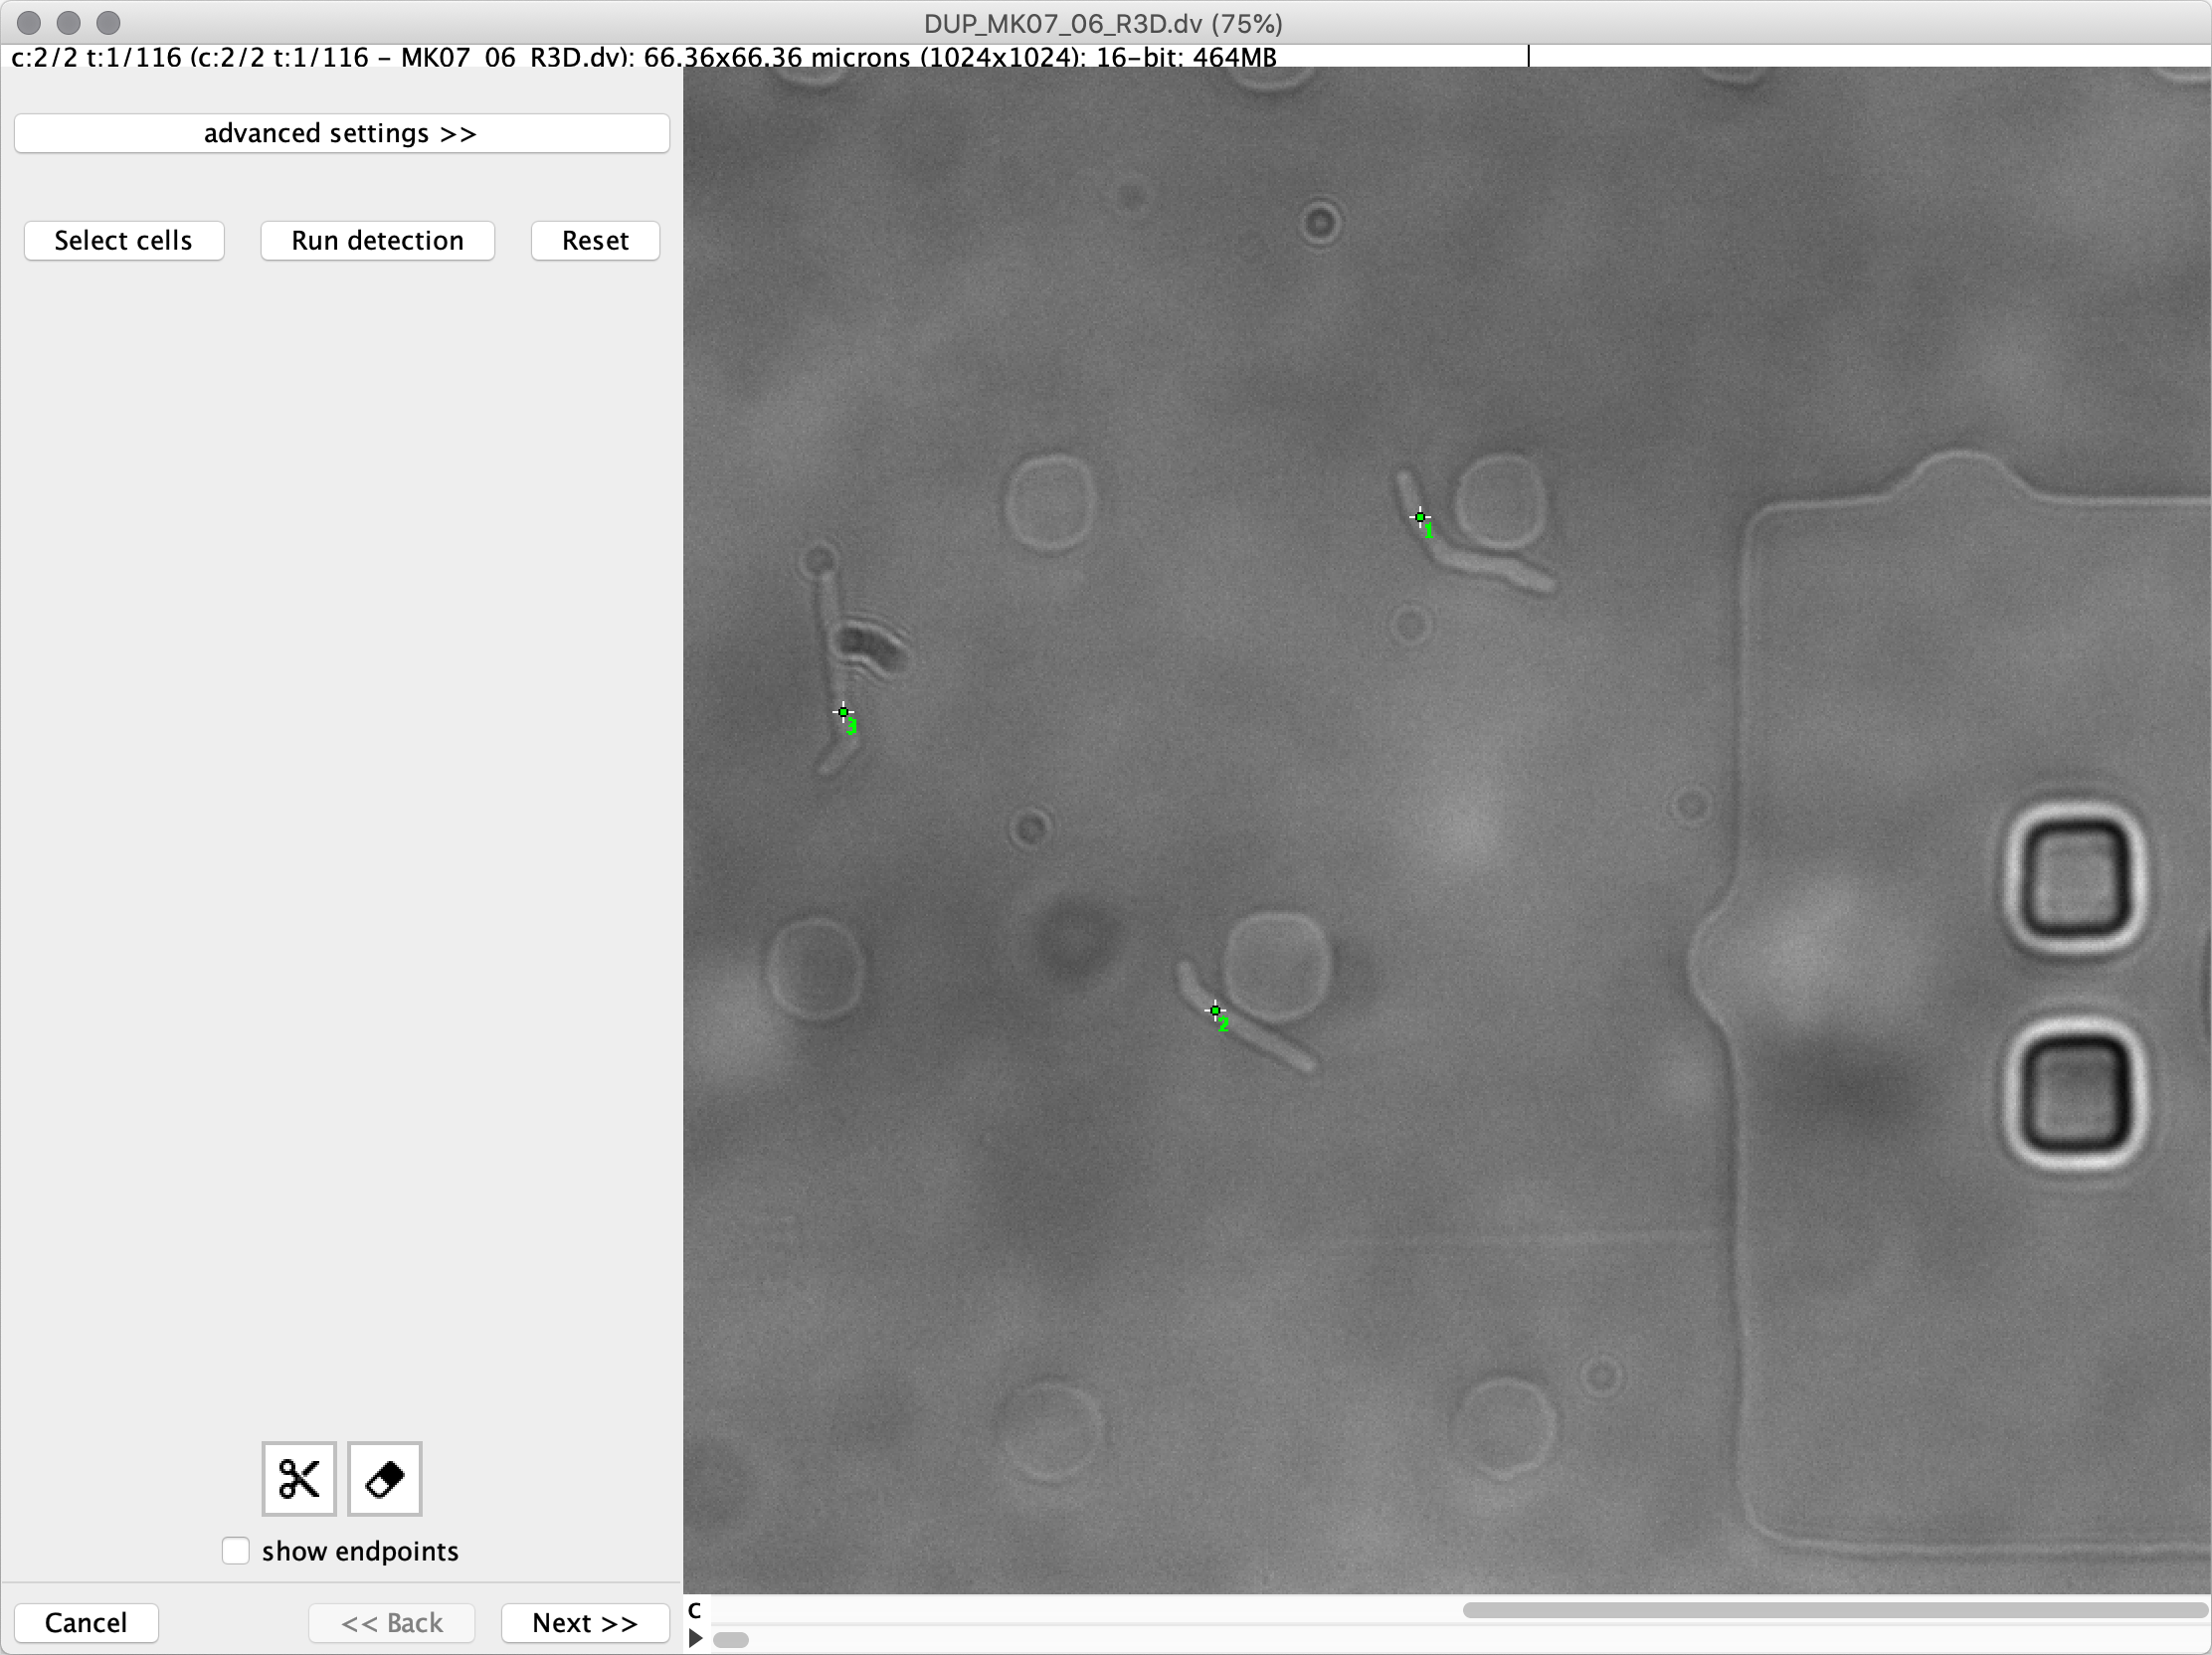
\includegraphics[width=\textwidth]{images/ui-step-detector.png}
  \caption{Pierwszy krok pluginu służący do wstępnej detekcji komórek.}
  \label{fig:ui-step-detector}
\end{figure}

W dodatkowym panelu \texttt{advanced settings} ukryte zostały dodatkowe parametry sterujące procesem detekcji komórek (\ref{sec:cell-detection}), takie jak siła rozmycia gaussowskiego czy wartość progowa użyte na etapie wstępnego przetwarzania obrazu.
Można tam również włączyć podgląd mapy indeksów kształtu, a także szkieletu na podstawie których przebiega proces detekcji.

\subsection{Śledzenie komórek w czasie}

Kolejnym krokiem jest śledzenie komórek w czasie (rysunek \ref{fig:ui-step-tracker}).
Użytkownik na tym etapie może zdecydować w jaki sposób chce dalej pracować.
Może skorzystać z opcji automatycznego wyliczenia jednej bądź kilku kolejnych klatek (przycisk \texttt{calculate next}) lub zduplikować aktualnie zaznaczone komórki do kolejnej klatki a następnie skorzystać z dostępnych narzędzi i manualnie je dostosować (\texttt{duplicate}).
Cofając się w historii do poprzednich klatek można poprawiać zaznaczenia. Można też powtórnie wyliczyć zaznaczenia na danym obrazie, jednak należy wtedy pamiętać, że zaznaczenia w kolejnych klatkach zostaną zresetowane.

\begin{figure}
  \centering
  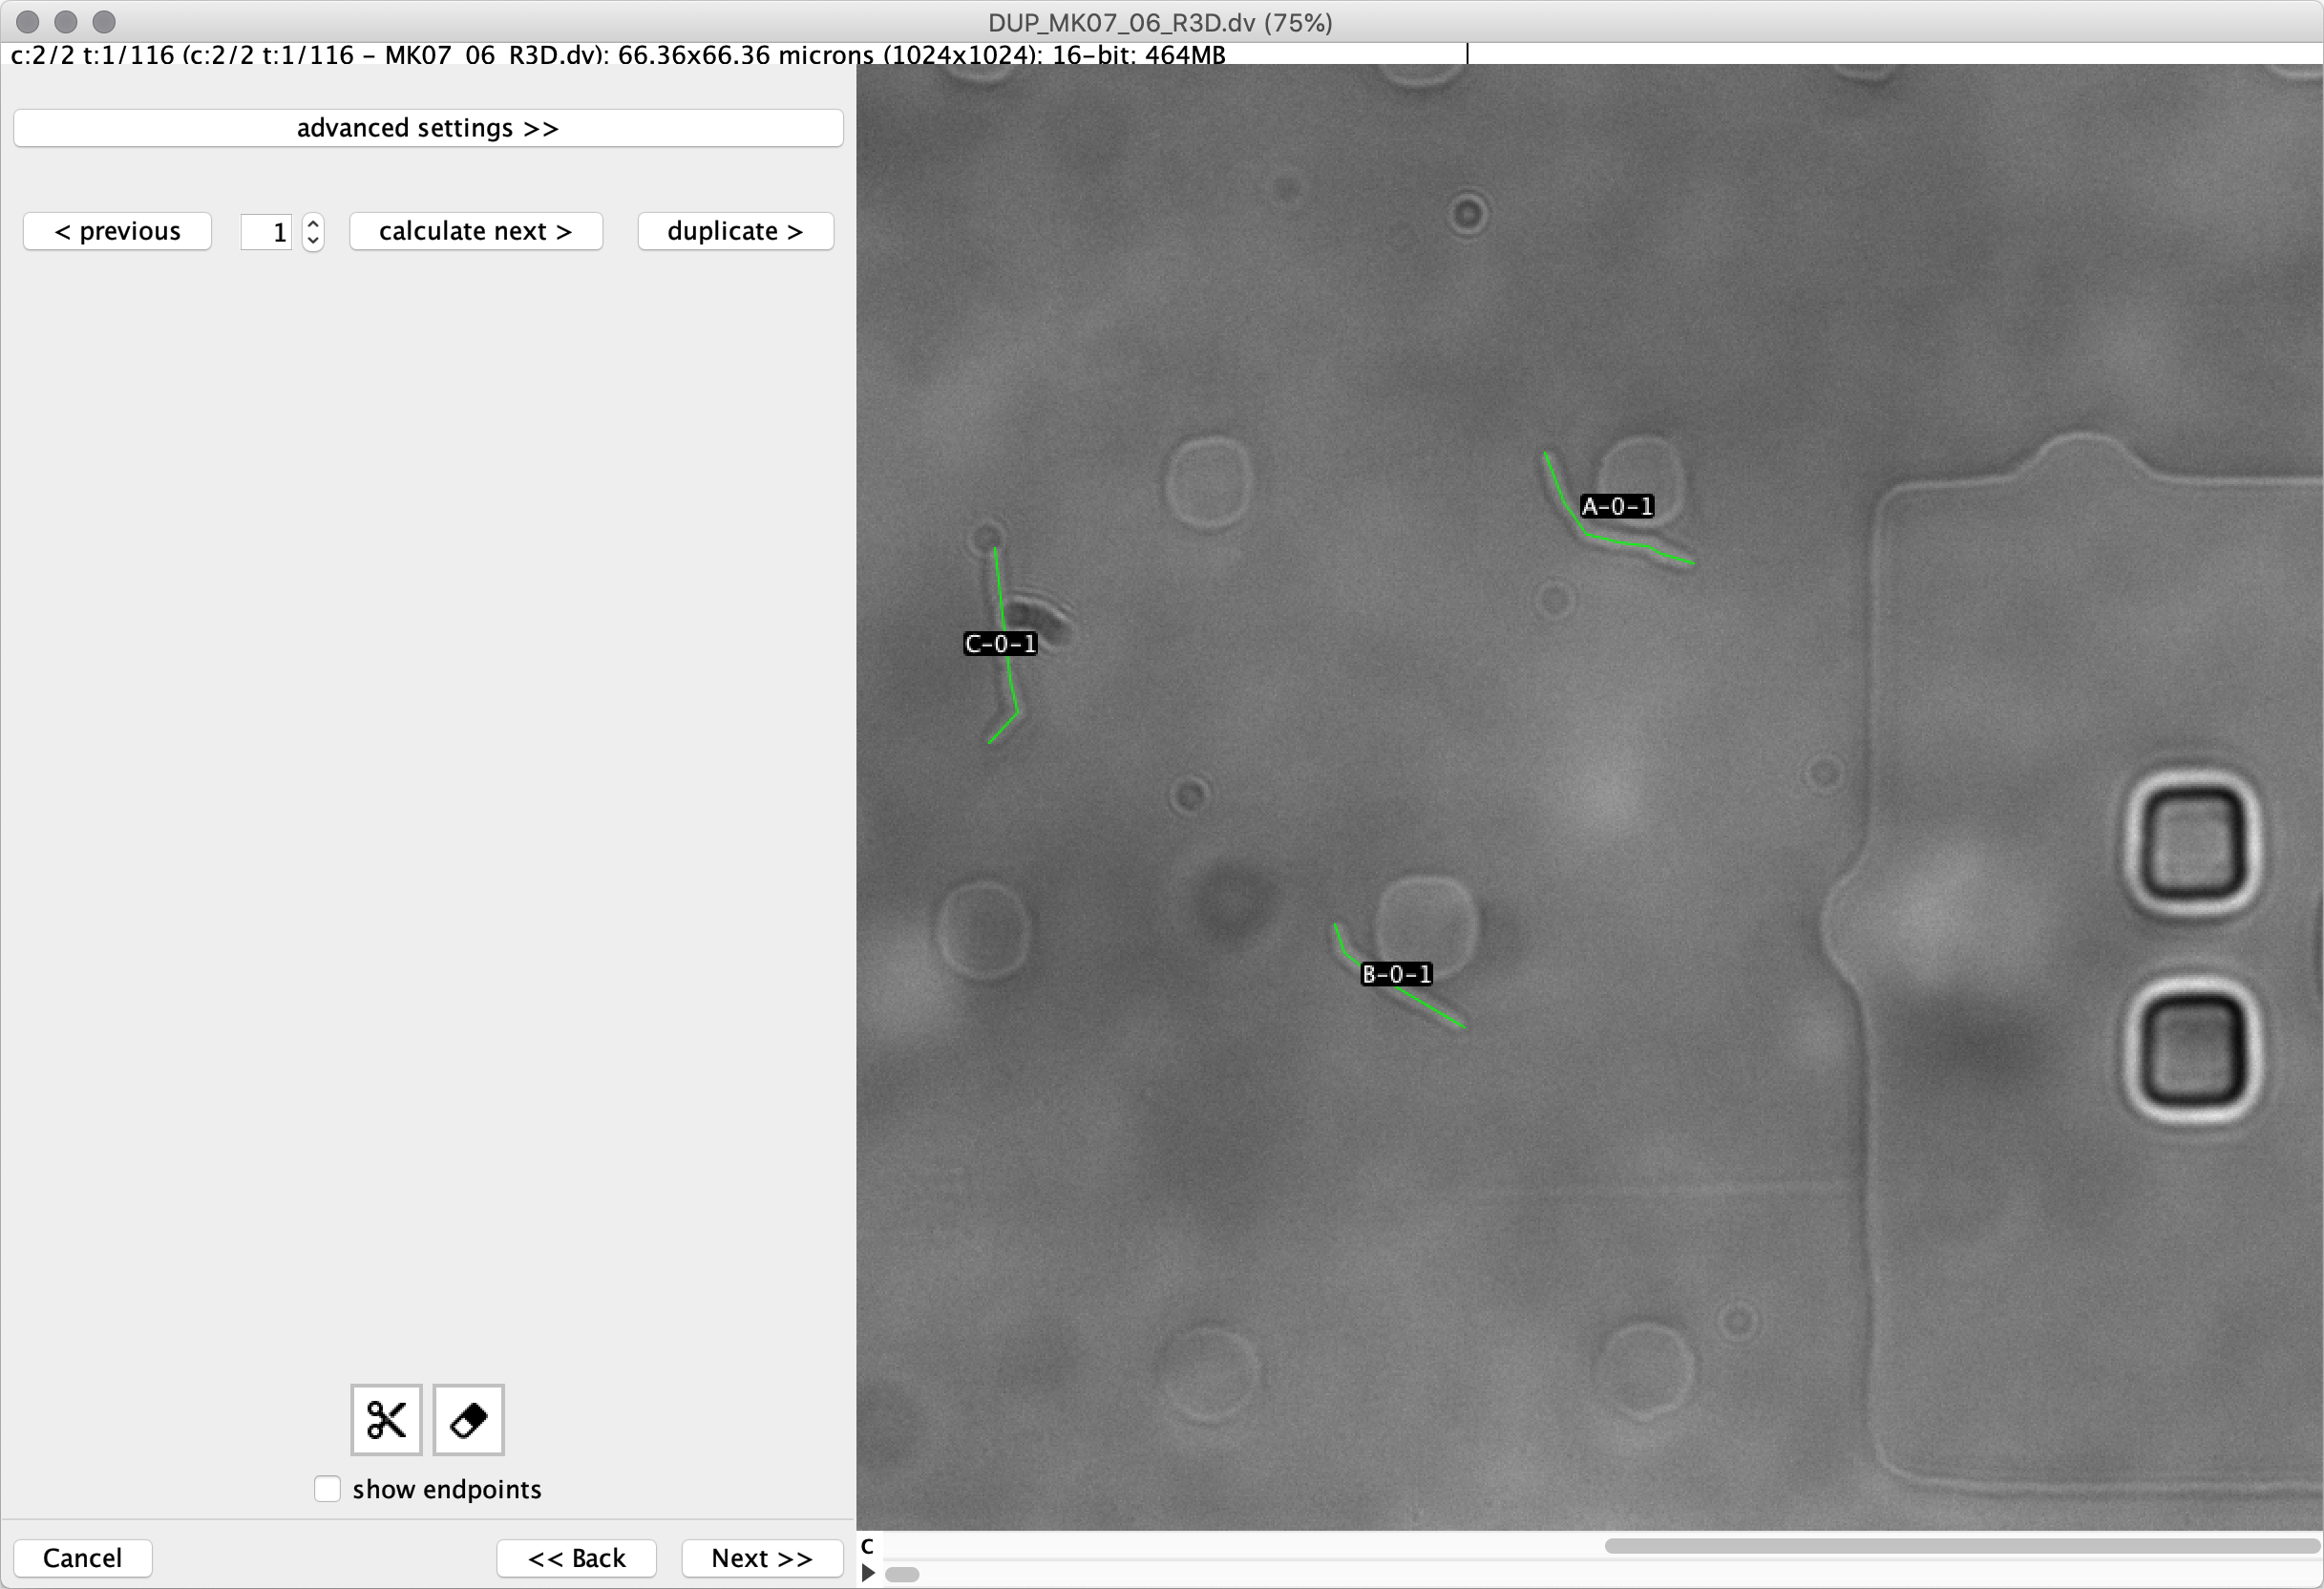
\includegraphics[width=\textwidth]{images/ui-step-tracker.png}
  \caption{Drugi krok pluginu służący do wstępnej śledzenia komórek w czasie.}
  \label{fig:ui-step-tracker}
\end{figure}

\subsection{Analiza danych}

\begin{figure}
  \centering
  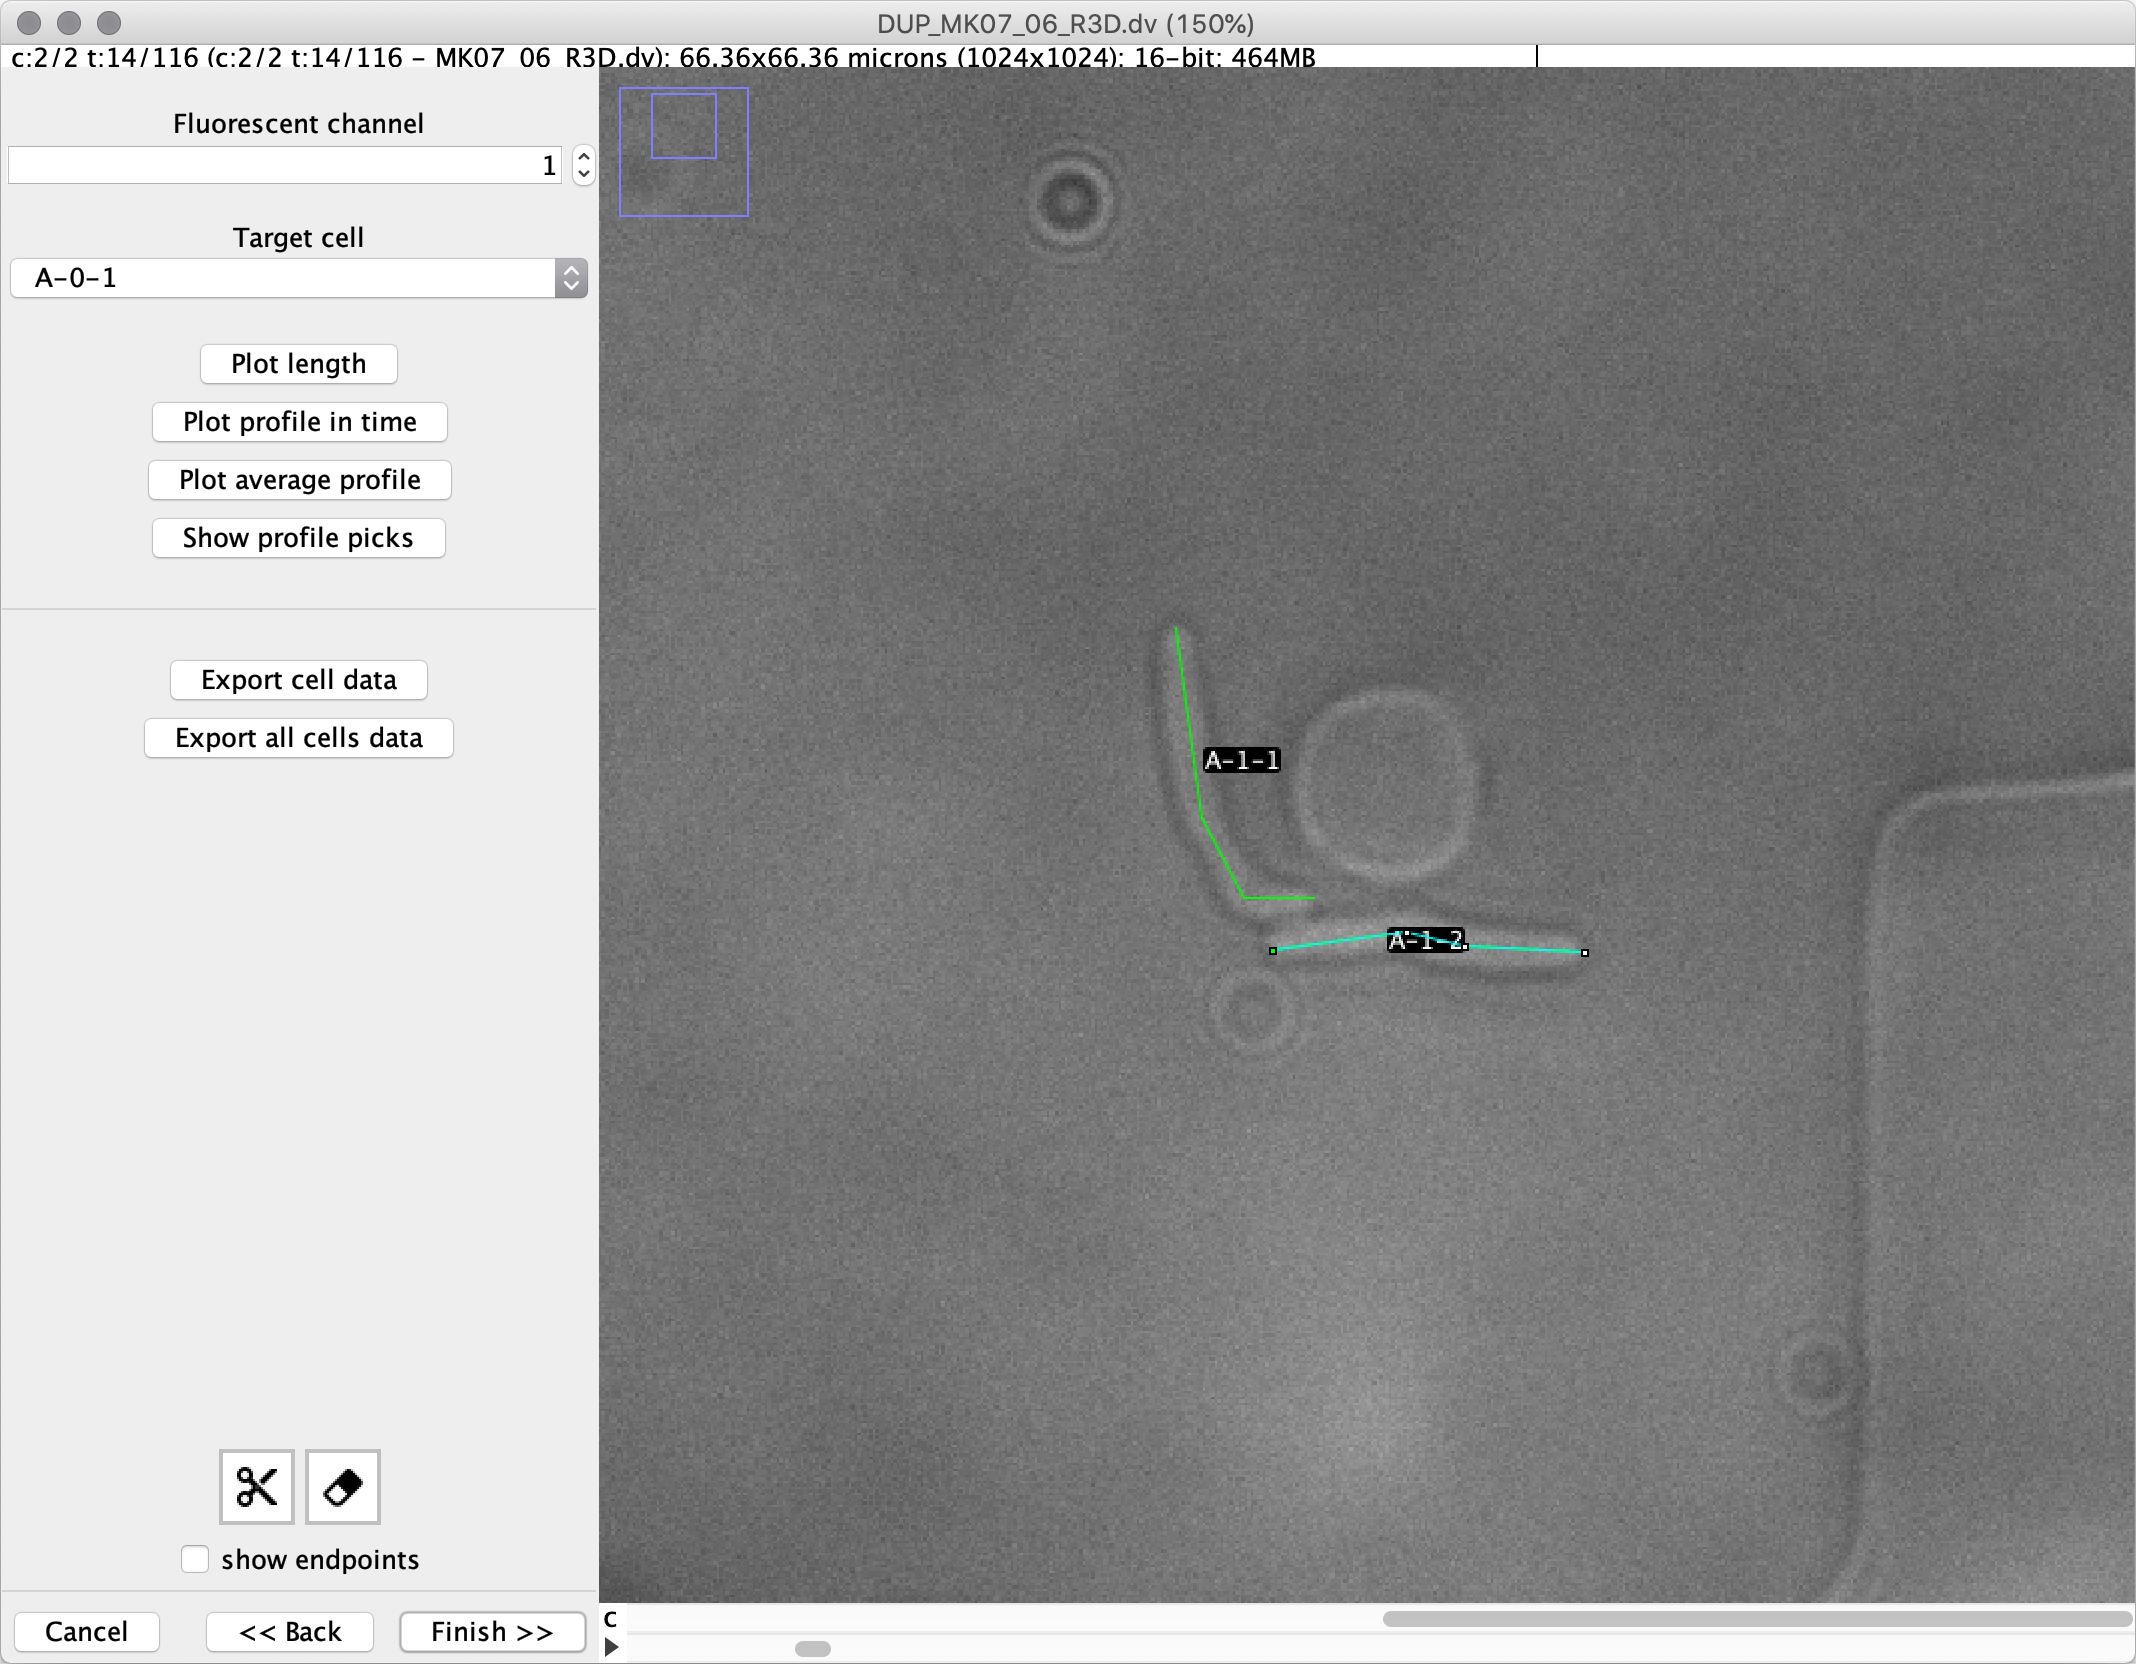
\includegraphics[width=\textwidth]{images/ui-step-measurements.png}
  \caption{Trzeci krok pluginu służący do analizy zaznaczonych komórek.}
  \label{fig:ui-step-measurements}
\end{figure}

Ostatni krok umożliwia analizę danych wyliczonych na podstawie zaznaczonych komórek (rysunek \ref{fig:ui-step-measurements}).
W celu zapewnienia poprawności danych należy najpierw wskazać numer kanału z fluorescencją. Kolejnym krokiem jest wybór komórki do analizy.
Umieszczona niżej sekcja przycisków pozwala na wyświetlenie kilku rodzajów wykresów (rysunek \ref{fig:ui-plots}):

\begin{itemize}
  \item wykresu przedstawiającego zmianę długości w czasie
  \item stosu profili intensywności pod łamaną opisującą komórkę na kanale z fluorescencją (dla każdej klatki życia komórki)
  \item średniego profilu intensywności od łamaną opisującą komórkę na kanale z fluorescencją (oś X każdego profilu jest przed uśrednieniem normalizowana do przedziału $[0, 1]$)
  \item umiejscowienia ,,ognisk'' na kanale z fluorescencją w czasie.
\end{itemize}

\begin{figure}
  \centering
  
  \begin{subfigure}[t]{.45\textwidth}
    \centering
    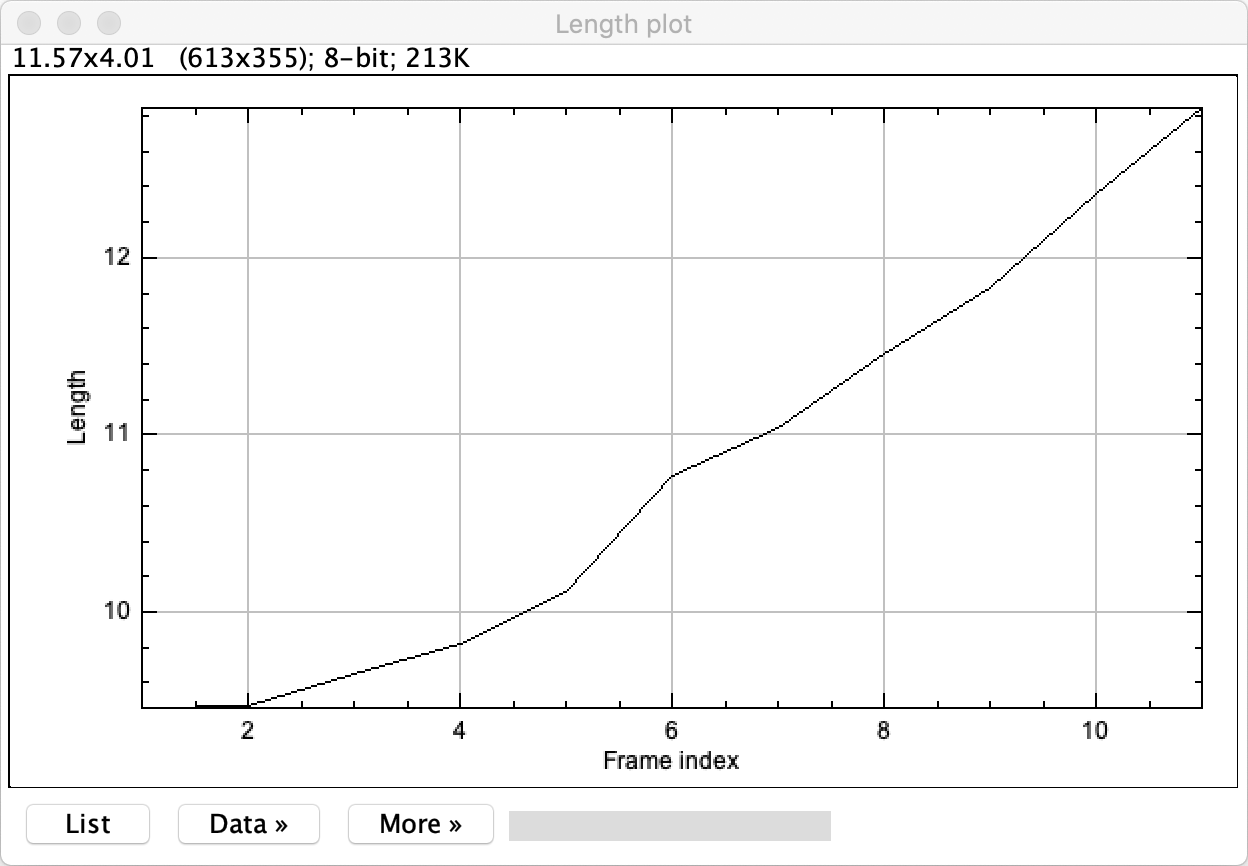
\includegraphics[width=\textwidth]{images/ui-plot-lengths.png}
    \caption{\centering Wykresu przedstawiający zmianę długości w czasie.}
  \end{subfigure}
  \hfill
  \begin{subfigure}[t]{.45\textwidth}
    \centering
    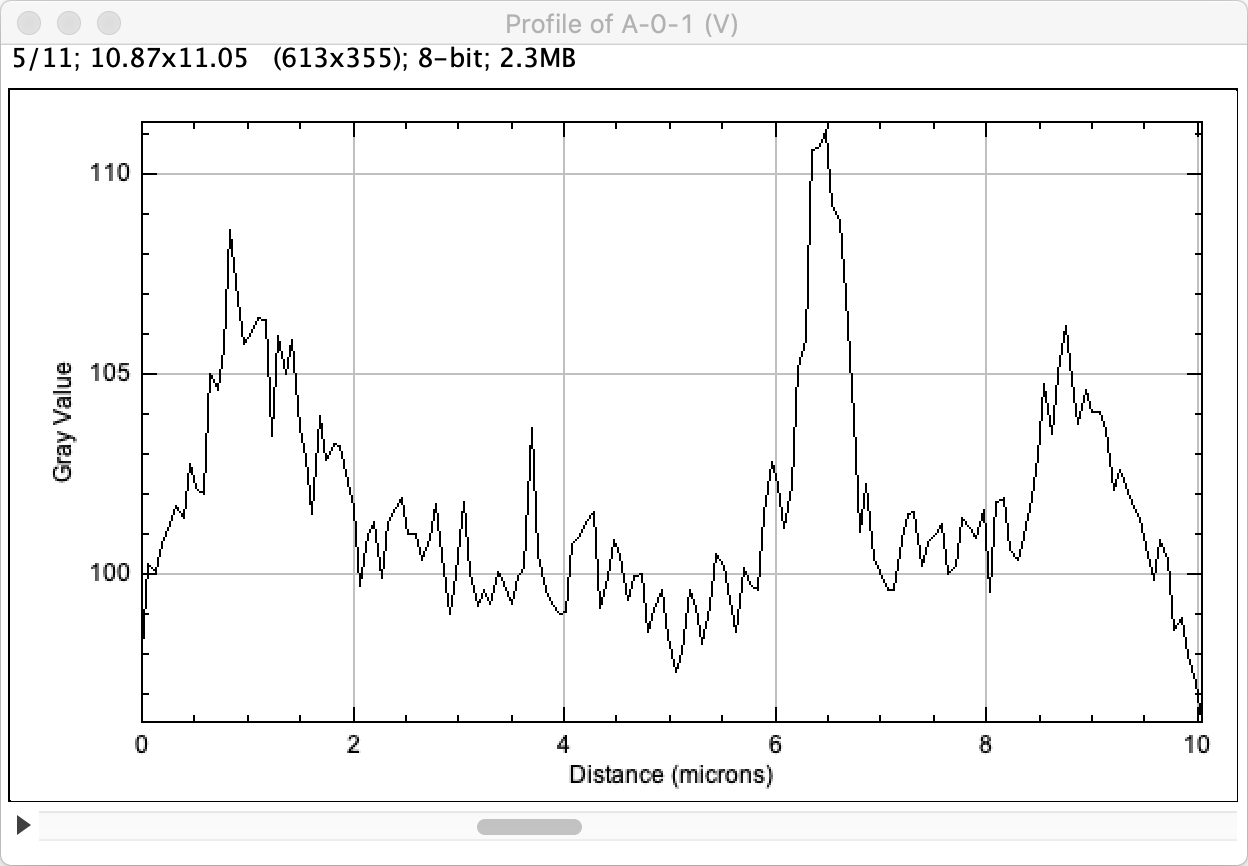
\includegraphics[width=\textwidth]{images/ui-plot-profiles.png}
    \caption{\centering Stos profili intensywności pod łamaną opisującą komórkę na kanale z fluorescencją.}
  \end{subfigure}
  \hfill
  
  \par\bigskip
  
  \begin{subfigure}[t]{.45\textwidth}
    \centering
    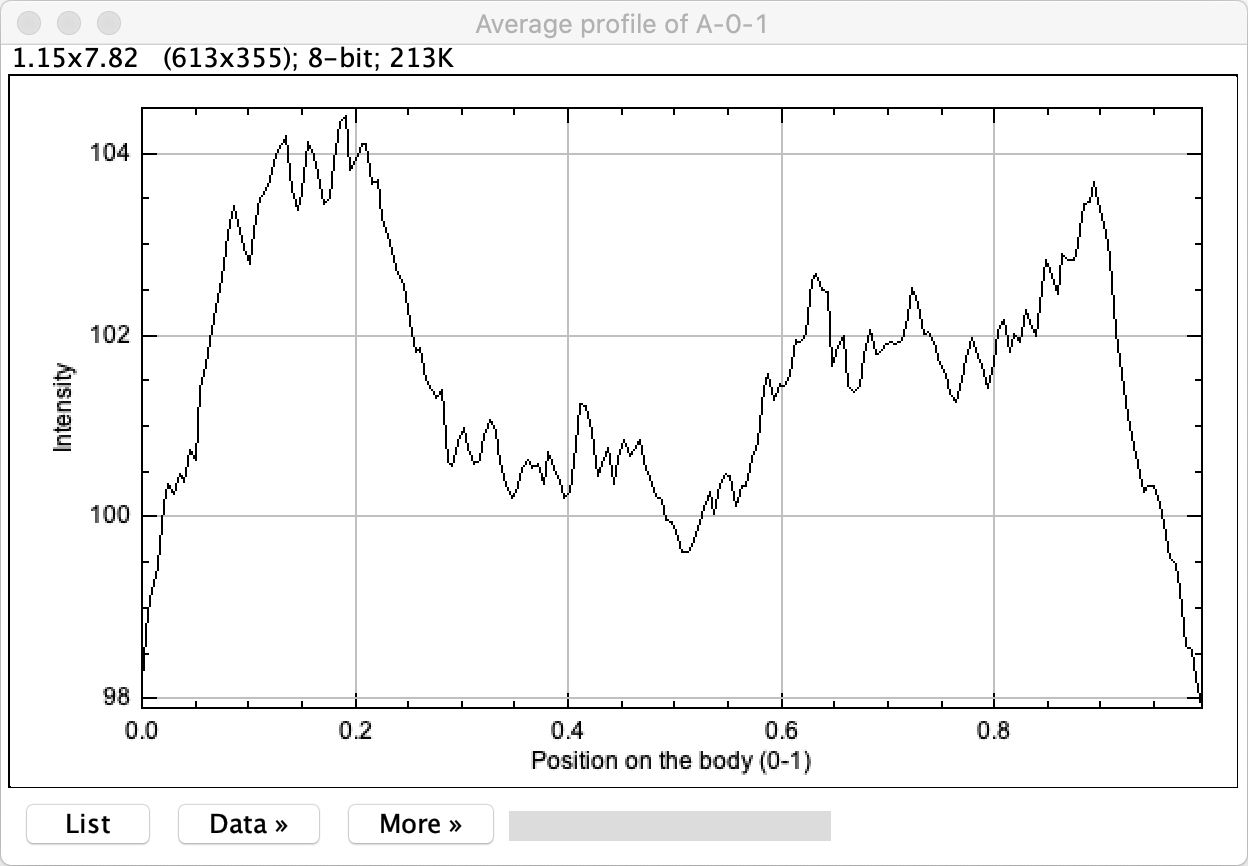
\includegraphics[width=\textwidth]{images/ui-plot-avg-profile.png}
    \caption{\centering Średni profil intensywności od łamaną opisującą komórkę na kanale z fluorescencją.}
  \end{subfigure}
  \hfill
  \begin{subfigure}[t]{.45\textwidth}
    \centering
    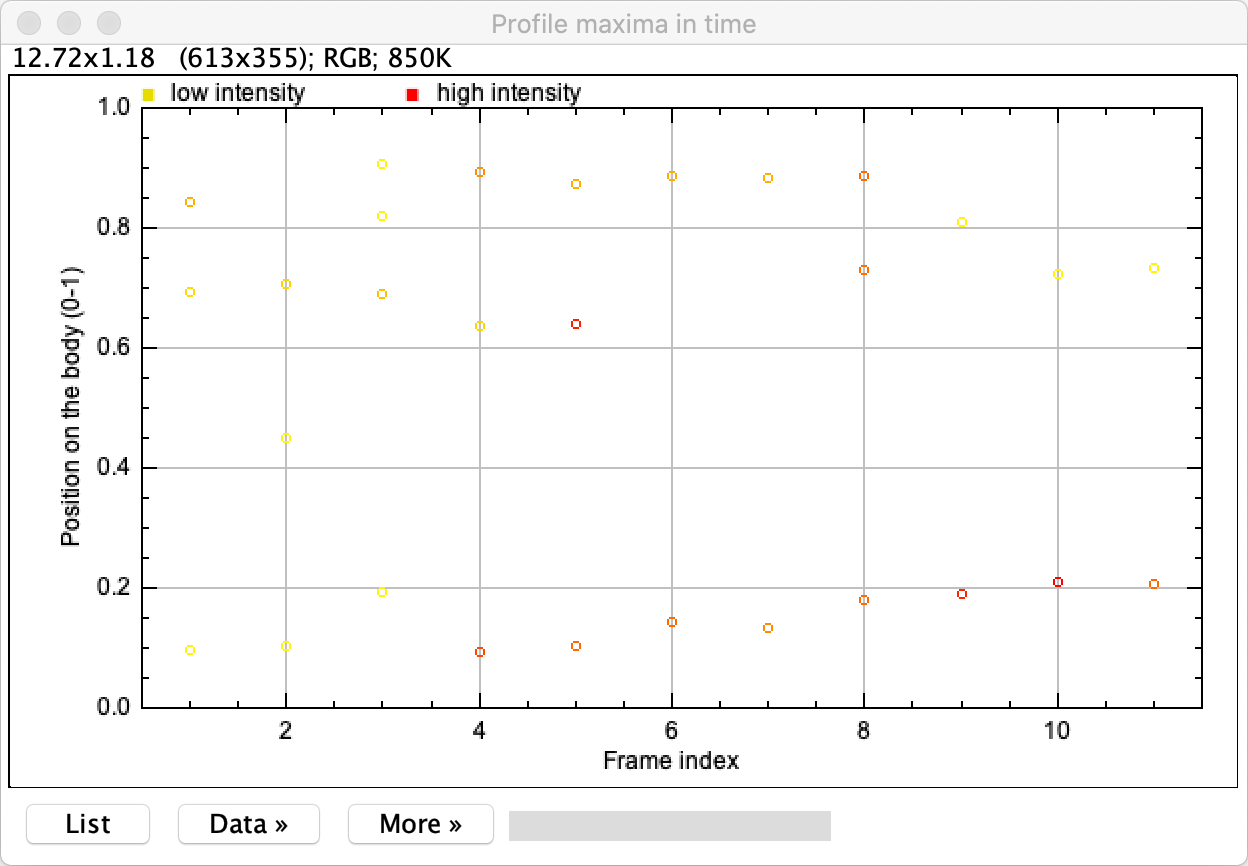
\includegraphics[width=\textwidth]{images/ui-plot-picks.png}
    \caption{\centering Umiejscowienie ,,ognisk'' na kanale z fluorescencją w czasie.}
  \end{subfigure}
  \hfill
  
  \caption{Różne rodzaje wykresów.}
  \label{fig:ui-plots}
\end{figure}

W celu analizy profili i długości komórek poza programem można, za pomocą kolejnych przycisków, wyeksportować dane pojedynczej lub wszystkich komórek do formatu \texttt{CSV} (ang. comma-separated values).


\subsection{Manualna modyfikacja komórek}
\label{sec:user-manual-modifications}

W celu manualnej modyfikacji komórki należy wybrać ją w oknie \texttt{ROI Manager}, które otwierane jest automatycznie podczas pracy z komórkami (rysunek \ref{fig:ui-roi-manager}).
Komórka na obrazie będzie wyświetlona w postaci standardowego zaznaczenia wykonanego narzędziem do zaznaczania linii łamanej (ang. Segmented Line Selection Tool)\cite{imagej:segmented-line}.
Przesuwanie, usuwanie lub dodawanie wierzchołków takiego zaznaczenia zapisywane jest także dla komórki.
Komórki usunięte z listy okna \texttt{ROI Manager} zostaną usunięte również z kolekcji wraz z zaznaczeniami w kolejnych klatkach, jak i całym potomstwem.
Kolekcja zaznaczeń dla poprzednich klatek pozostanie bez zmian.

\begin{figure}
  \centering
  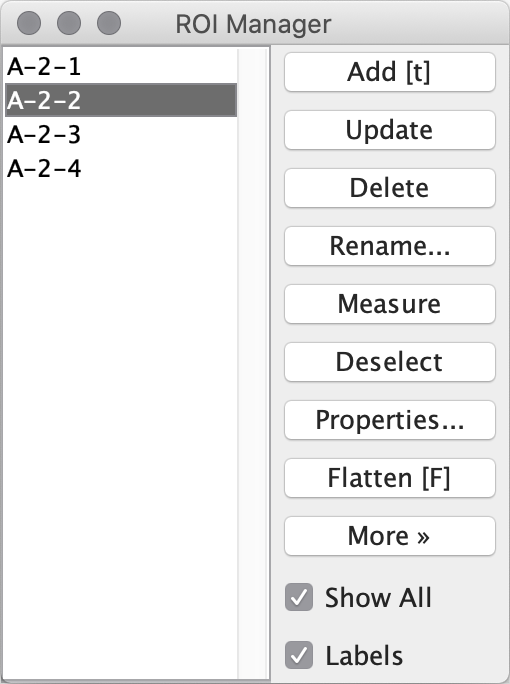
\includegraphics[width=0.3\textwidth]{images/ui-roi-manager.png}
  \caption{Okno \texttt{ROI Manager} pozwalające na wybór komórki.}
  \label{fig:ui-roi-manager}
\end{figure}

Dodatkowo okno pluginu wyposażone jest w dwa dodatkowe narzędzia mające ułatwić manualną edycję komórek. Narzędzia można włączyć za pomocą przycisków widocznych w lewym dolnym rogu okna pluginu.

Tryb rozcinania komórek można aktywować za pomocą przycisku z ikoną w kształcie nożyczek (\raisebox{-0.1em}{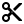
\includegraphics[width=0.9em]{images/tool-cut.png}}).
Służy on do ręcznego oznaczania punktów podziału komórek. Po jego uruchomieniu użytkownik może ,,przeciąć'' komórkę rysując symboliczną linię na obrazie.
Przecięta komórka zostanie podzielona na dwie komórki, które zostaną dodane do kolekcji jako ,,dzieci'' komórki sprzed podziału (jeśli występuje ona w poprzedniej klatce).
Ze względu na cykl życia opisywanych komórek, nie jest możliwe doprowadzenie do stanu w którym jedna komórka dzieli się na więcej niż dwie części.
Należy pamiętać, że rozcięcie komórki, która została oznaczona w późniejszych klatkach, wiąże się z utratą jej zaznaczeń w tych klatkach oraz usunięciem jej potomstwa.

Drugim dodatkowym narzędziem jest tryb skracania końcówek, uruchamiany za pomocą przycisku z ikoną w kształcie gumki do mazania (\raisebox{-0.1em}{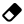
\includegraphics[width=0.9em]{images/tool-erase.png}}).
Działa on podobnie do narzędzia ,,gumki'' obecnego w popularnych programach graficznych. Za jego pomocą nie można podzielić komórki, ale można ją skrócić lub całkowicie usunąć.
Jeśli cała komórka zostanie ,,wymazana'' to, analogicznie jak przy usuwaniu komórki z poziomu okna \texttt{ROI Manager}, usunięte zostaną również zaznaczenia w kolejnych klatkach oraz jej potomstwo.

\subsection{Nazewnictwo komórek oraz ich orientacja}
\label{sec:cell-naming}

Aby ułatwić identyfikację komórek, przyjąłem stałą konwencję ich nazewnictwa.
Nazwa składa się z trzech członów: identyfikatora komórki źródłowej, indeksu pokolenia oraz indeksu w ramach pokolenia.
Komórkom źródłowym (nie mającym rodzica) zostaje przydzielony unikalny identyfikator w postaci wielkiej litery alfabetu.
Indeks pokolenia jak i indeks w ramach pokolenia wynikają z natury kolekcji komórek.
Każda komórka dzieli się w pewnym momencie na dwie nowe komórki (dzieci) nowego pokolenia.
,,Drzewo genealogiczne'' komórek będzie w takim przypadku drzewem binarnym, a indeksy pokolenia i w ramach pokolenia będą odpowiednio odległością od korzenia i liczbą porządkową w ramach tego samego indeksu pokolenia.
Przykładowe drzewo pokrewieństwa opisane nazwami komórek przedstawia rysunek \ref{fig:tree-naming}.


\begin{figure}[h]
  \Tree 
    [.\texttt{A-0-1}
      [.\texttt{A-1-1}
        [.\texttt{A-2-1}
          {\ldots}
          {\ldots}
        ]
        [.\texttt{A-2-2}
          {\ldots}
          {\ldots}
        ]
      ]
      [.\texttt{A-1-2}
        [.\texttt{A-2-3}
          {\ldots}
          {\ldots}
        ]
        [.\texttt{A-2-4}
          {\ldots}
          {\ldots}
        ]
      ]
    ]
  \caption{Drzewo genealogiczne opisane zgodnie z konwencją nazewnictwa.}
  \label{fig:tree-naming}
\end{figure}

Dzięki tak skonstruowanej konwencji nazewnictwa można łatwo zidentyfikować pochodzenie komórki, a także stopień pokrewieństwa z innymi komórkami.

W celu zapewnienia spójności analizowanych na końcu danych, ustaliłem również stałą orientację komórek.
Aby móc rozróżnić końcówki komórek, wystarczy zaznaczyć opcję \texttt{show endpoints} w dolnej części okna pluginu.
Kolorem czerwonym oznaczone zostaną końcówki powstałe w wyniku podziału komórki, a zielonym te które były wcześniej końcówkami komórki rodzica (rysunek \ref{fig:ui-show-endpoints}). W przypadku komórki źródłowej końcówki oznaczone są losowo.

\begin{figure}
  \centering
  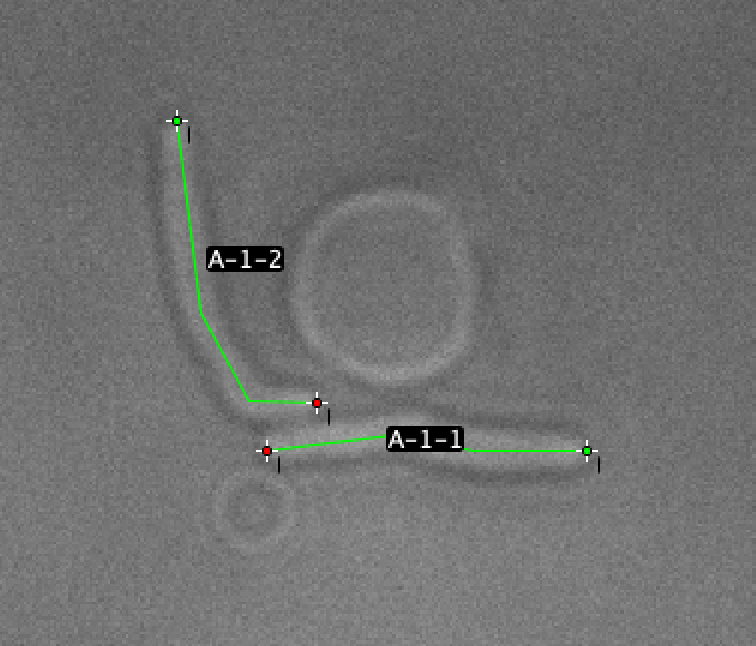
\includegraphics[width=0.3\textwidth]{images/ui-show-endpoints.png}
  \caption{Komórki wraz ze znacznikami identyfikującymi końcówki.}
  \label{fig:ui-show-endpoints}
\end{figure}

\subsection{Importowanie i eksportowanie komórek}

Manualne oznaczanie i poprawianie komórek może być czasochłonne i nie zawsze można zakończyć pracę w ciągu jednej sesji.
Aby nie utracić efektów swojej pracy, użytkownik może wyeksportować oznaczone komórki za pomocą menu \texttt{Development > Export cells}.
Stworzony w ten sposób plik \texttt{XML} jest wynikiem serializacji kolekcji komórek.
Podczas kolejnej sesji, po otwarciu tego samego nagrania, zapisane komórki można wczytać korzystając z menu \texttt{Development > Import cells}.

\section{Dokumentacja techniczna}

\subsection{Struktura projektu}

Główna struktura plików projektu podzielona jest zgodnie z konwencją zaproponowaną przez zespół Apache Maven\cite{docs:maven-project-layout}. Główne foldery to:
\begin{itemize}
  \item \texttt{src/main/java} -- kod źródłowy aplikacji
  \item \texttt{src/main/resources} -- zasoby aplikacji np. obrazki
  \item \texttt{src/test/java} -- kod źródłowy testów automatycznych.
\end{itemize}

Kod źródłowy aplikacji podzielony jest na kilka folderów, ze względu na aspekt którego dotyczy:

\begin{itemize}
  \item \texttt{cells} -- kod zawierający logikę dotyczącą domeny pracy, m.in. kod pluginu, interfejsy poszczególnych kroków, główne algorytmy itp.; wewnątrz wydzielono jeszcze dodatkowo foldery: 
  \begin{itemize}
    \item[$\circ$] \texttt{serialization} -- kod dotyczący importu i eksportu komórek
    \item[$\circ$] \texttt{skeleton} -- implementacja króków detekcji i śledzenia komórek opisana w tej pracy (oparta na szkieletyzacji)
    \item[$\circ$] \texttt{measurements} -- implementacja etapu analizy danych
  \end{itemize}
  \item \texttt{graph} -- implementacja grafu
  \item \texttt{gui} -- implementacje generycznych okien i komponentów interfejsu
  \item \texttt{imagej} -- klasy ułatwiające prace i komunikację z programem--hostem ImageJ
  \item \texttt{util} -- inne pomocnicze klasy
  \item \texttt{vendor} -- publicznie dostępne wtyczki do programu ImageJ lub opakowania ułatwiające korzystanie z zależności zadeklarowanych w \texttt{pom.xml}.
\end{itemize}

\subsubsection{Konwencja nazewnictwa}

Nazwy interfejsów rozpoczynają się od wielkiej litery ,,\texttt{I}'' np. \texttt{ICellsPluginStep}, natomiast nazwy klas abstrakcyjnych zaczynają się od prefiksu ,,\texttt{Abstract}'' np. \texttt{AbstractCellCollection}.

\subsection{Główne struktury danych}

\subsubsection{\texttt{AbstractCellCollection}}

Ta abstrakcyjna klasa służy do opisywania drzewiastej struktury komórek. Dziedziczą po niej dwie klasy: \texttt{CellCollection} oraz \texttt{Cell}.
Ta pierwsza służy do przechowywania kolekcji komórek reprezentowanych przez klasę \texttt{Cell}.
Druga natomiast oprócz reprezentowania komórki, może zawierać także referencje do dwóch komórek potomnych, tworząc w ten sposób binarne ,,drzewo genealogiczne'' komórki.

Klasa deklaruje m.in. metody dodawania i usuwania komórek z kolekcji, ale także metody do wydobywania wszystkich komórek ,,żyjących'' w danej klatce nagrania.

Klasy dziedziczące po \texttt{AbstractCellCollection} muszą być serializowalne.
Własność ta jest wykorzystywana podczas importowania i eksportowania komórek do pliku \texttt{XML}.

\subsubsection{\texttt{Cell}}

Jest to klasa opisująca komórkę i cały jej cykl życia -- od pojawienia się, do momentu podziału na dwie nowe komórki (może zawierać także referencje do tych komórek potomnych).
Obiekt tej klasy zawiera informacje o każdej klatce w której występuje komórka w postaci referencji do instancji \texttt{AbstractCellFrame}.
Pozwala też określić i odczytać poszczególne części nazwy komórki takie jak identyfikator komórki źródłowej, indeks pokolenia czy indeks w ramach pokolenia (\ref{sec:cell-naming}).

Poza wyżej wymienionymi oraz dziedziczonymi po klasie \texttt{AbstractCellCollection} funkcjonalnościami, obiekt tej klasy zawiera również metody potrzebne do uzyskania reprezentacji komórki w postaci standardowego zaznaczenia w programie ImageJ.

\subsubsection{\texttt{AbstractCellFrame}}

Klasa ta deklaruje metody służące do uzyskania zaznaczenia pojedynczej komórki w konkretnej klatce nagrania, a także do modyfikacji tego zaznaczenia.

Na potrzeby tej pracy powstała jej implementacja \texttt{PolylineCellFrame}, która reprezentuje zaznaczenie komórki w postaci linii łamanej.

\subsubsection{\texttt{Graph}, \texttt{Edge}, \texttt{Vertex}, \texttt{Point}}

Klasy te składają się na implementację grafu, który zawiera dodatkowe informacje o punktach składających się na krawędzie i wierzchołki.

\subsection{Architektura umożliwiająca dalszy rozwój}

Główną klasą projektu jest \texttt{CellsPlugin}, która instancjonowana jest przez program ImageJ po otwarciu wtyczki z poziomu menu \texttt{Development > Cell Detector}.
Podczas uruchomienia tworzona jest kopia aktualnie otwartego stosu obrazów, która wyświetlona zostaje w specjalnym oknie pluginu (jego opis znajduje się w rozdziale \ref{sec:user-manual}), a także utworzona zostaje pusta kolekcja komórek.

Podczas inicjalizacji uruchomiony zostaje również nasłuch na różnego rodzaju zdarzenia programu--hosta ImageJ m.in. na:
\begin{itemize}
  \item zmiany podglądu obrazu -- umożliwia to wyświetlenie odpowiednich komórek dla aktualnie oglądanej klatki
  \item zmiany zaznaczeń na obrazie -- dzięki temu zmiany mogą być zapisywane dla komórek opisywanych przez zmodyfikowane zaznaczenia
  \item zmianę aktywnego narzędzia -- może mieć wpływ na zachowanie wybranego narzędzia specjalnego (\ref{sec:user-manual-modifications})
  \item zmiany na liście okna \texttt{Roi Manager} -- umożliwia to usuwanie komórek z poziomu tego okna.
\end{itemize}

Każdy z trzech etapów pluginu (wstępna detekcja, śledzenie komórek i analiza danych) jest obiektem klasy implementującej interfejs \texttt{ICellsPluginStep}.
Interfejs ten deklaruje zaledwie trzy publiczne metody:

\begin{itemize}

\item \texttt{JComponent init(ImagePlus imp, CellCollection cells)}

Metoda ta wywoływana jest podczas inicjalizacji danego kroku np. przy starcie pluginu (dla kroku wstępnej detekcji) lub przy wciśnięciu przycisku \texttt{next} (dla kolejnego kroku).
Argumentami są obraz źródłowy (nagranie) oraz referencje do kolekcji komórek.
Metoda odpowiedzialna jest również za stworzenie i zwrócenie komponent interfejsu danego kroku, który zostanie automatycznie umieszczony w odpowiednim miejscu okna wtyczki.

\item \texttt{void imageUpdated()}

Ta metoda służy do nasłuchiwania na zmiany obrazu i wyświetlanych komórek.
Uruchamiana jest przez przez plugin po każdej aktualizacji podglądu obrazu i komórek na nim wyświetlonych.

\item \texttt{void cleanup()}

Metoda ta wywoływana jest podczas zmiany aktualnego kroku lub przy zamknięciu pluginu.

\end{itemize}

Dzięki tak zaprojektowanemu systemowi każdy z etapów programu jest niezależny i może zostać z łatwością wymieniony na inną implementację tego interfejsu.
Kod pluginu zawiera wszystkie główne struktury danych (lub ich abstrakcyjne wersje) i dzięki temu jest zupełnie niezależny od implementacji poszczególnych kroków -- komunikuje się z nimi jedynie za pomocą opisanych wyżej interfejsów.
Funkcjonalności niezależne od implementacji poszczególnych etapów takie jak wyświetlanie, usuwanie i ręczna modyfikacja komórek, a także ich eksportowanie i importowanie, bazują wyłącznie na metodach deklarowanych przez odpowiednie interfejsy lub klasy abstrakcyjne.

\subsection{Wykorzystywane API ImageJ}

\ldots % TODO Opis wykorzystanego API ImageJ

\subsection{Błędy w implementacji ImageJ i sposoby na ich obejście}
\ldots % TODO Błędy w implementacji ImageJ i sposoby na ich obejście

\subsection{Opis sposobu dalszego rozwoju, interfejsy}
\ldots % TODO Opis sposobu dalszego rozwoju, interfejsy


%%%%%%%%%%%%%%%%%%%%%%%%%%%%%%%%%%%%%%%%%%%%%%%%%%%%%%%%%%%%%%%%%%%%%%%%%%%%%%%%%%%%%%%%%%%

\chapter{Zakończenie}

%%%%%%%%%%%%%%%%%%%%%%%%%%%%%%%%%%%%%%%%%%%%%%%%%%%%%%%%%%%%%%%%%%%%%%%%%%%%%%%%%%%%%%%%%%%


\section{Podsumowanie}
\ldots % TODO Podsumowanie
\section{Ograniczenia wynikające z zastosowanych metod}
\ldots % TODO Ograniczenia wynikające z zastosowanych metod
\section{Dalszy rozwój}
\ldots % TODO Dalszy rozwój


%%%%%%%%%%%%%%%%%%%%%%%%%%%%%%%%%%%%%%%%%%%%%%%%%%%%%%%%%%%%%%%%%%%%%%%%%%%%%%%%%%%%%%%%%%%

%%%%% BIBLIOGRAFIA

%%%%%%%%%%%%%%%%%%%%%%%%%%%%%%%%%%%%%%%%%%%%%%%%%%%%%%%%%%%%%%%%%%%%%%%%%%%%%%%%%%%%%%%%%%%


%\bibitem{example} \ldots

\begin{thebibliography}{1}

\bibitem{paper:shape-index}
  Jan J Koenderink, Andrea J van Doorn,
  \emph{Surface shape and curvature scales},
  Image and Vision Computing,
  10:557--565,
  1992.

\bibitem{plugin:shape-index-map}
  Johannes Schindelin,
  \emph{Shape Index Map},
  2010,
  \url{https://imagej.net/Shape_Index_Map}.

\bibitem{algo:3d-thinning}
  Ta-Chih Lee, Rangasami L. Kashyap, Chong-Nam Chu,
  \emph{Building skeleton models via 3-D medial surface/axis thinning algorithms},
  Computer Vision, Graphics, and Image Processing,
  56(6):462--478,
  1994.

\bibitem{plugin:skeletonize-3d}
  Ignacio Arganda-Carreras,
  \emph{Skeletonize3D},
  2.1.1,
  2017,
  \url{https://imagej.net/Skeletonize3D}.

\bibitem{plugin:analyze-skeleton}
  Ignacio Arganda-Carreras,
  \emph{AnalyzeSkeleton},
  3.3.0,
  2018,
  \url{https://imagej.net/AnalyzeSkeleton}.
  
\bibitem{algo:ramer-douglas-peucker}
  Wikipedia,
  \emph{Ramer--Douglas--Peucker algorithm},
  \url{https://en.wikipedia.org/wiki/Ramer-Douglas-Peucker_algorithm}.
  
\bibitem{imagej:segmented-line}
  ImageJ User Guide,
  \emph{Segmented Line Selection Tool},
  \url{https://imagej.nih.gov/ij/docs/guide/146-19.html#sub:Segmented-Line-Selection}.
  
\bibitem{docs:maven-project-layout}
  Apache Maven Project,
  \emph{Introduction to the Standard Directory Layout},
  \url{https://maven.apache.org/guides/introduction/introduction-to-the-standard-directory-layout.html}

\end{thebibliography}

\end{document}
